\documentclass[book,paper=a4,fontsize=11pt]{jlreq}
\usepackage[top=25mm,bottom=25mm,left=25mm,right=25mm]{geometry}
\usepackage{amsmath,amssymb}
\usepackage{xcolor}
\usepackage{graphicx}
\usepackage{placeins}
\usepackage{cite}
\usepackage[colorlinks=true,linkcolor=blue,citecolor=blue,urlcolor=blue]{hyperref}
\usepackage{bookstyle}

\title{宇宙線と空気シャワーの基礎}
\author{Ichiro KOMAE}
\hypersetup{
  pdftitle={宇宙線と空気シャワーの基礎},
  pdfauthor={Ichiro KOMAE}
}
% \date{}

\begin{document}
\frontmatter
\begin{titlepage}
    \sffamily
    \vspace*{4cm}

    \begin{flushleft}
        {\Large \textcolor{BookAccent}{\bfseries Cosmic Rays and Extensive Air Showers}}\par
        \vspace{1.5cm}

        \makeatletter
        {\fontsize{34pt}{42pt}\selectfont \bfseries \@title\par}
        \vspace{1.5cm}

        {\color{BookLine}\rule{0.8\textwidth}{1pt}}\par
        \vspace{1.5cm}

        {\Large \textcolor{BookAccent}{\bfseries \@author}}\par
        \makeatother
    \end{flushleft}

    \vfill

    \begin{center}
        \makeatletter
        {\large \textcolor{BookAccent}{\the\year/\two@digits{\month}/\two@digits{\day}}}
        \makeatother
    \end{center}
\end{titlepage}
\setcounter{tocdepth}{2}
\tableofcontents

\mainmatter

\chapter{宇宙線の観測と起源}\label{chap:cosmic_rays}
宇宙線は、宇宙空間から地球へ到来する高エネルギーの荷電粒子である。一次宇宙線の主成分は陽子とヘリウム原子核であり、より重い原子核も含まれる。
一次宇宙線が大気中の原子核と相互作用すると、多数の二次粒子からなる空気シャワーが発生する。地表での粒子密度と到来時刻、大気中での発光量と縦方向発達から、一次宇宙線のエネルギー、質量組成、到来方向を推定する~\cite{PDGCosmicRays,Stanev2004}。

本章では、全粒子エネルギースペクトルの軟化である second knee を中心に、観測された特徴と加速・伝搬による解釈を整理する。Second knee は鉄成分の軟化や銀河系内成分の終端と関係する可能性があるが、これらと同義ではない。スペクトル、質量組成、異方性による制約を合わせ、TALE の地表検出器による測定の目的へつなげる。

\section{宇宙線研究の成立}
20 世紀初頭、検電器の放電から空気のわずかな電離が知られ、その主因は地殻中の放射性物質が放つ放射線と考えられていた。しかし、Wulf の塔上での測定と Pacini の水中での遮蔽実験は、地殻からの放射だけでは説明できない寄与を示した~\cite{Carlson2012,HessTranslation2018}。
Victor Franz Hess は 1912 年に 7 回の気球飛行を行い、検電器で電離率の高度依存を測定した。図~\ref{fig:hess_altitude}に示す第 7 回飛行では、高度約 \(2\ \mathrm{km}\) を超えると電離率が増え、高高度では地上の約 2 倍に達した。Hess は、透過力の強い放射線が上方から大気へ入射していると結論した~\cite{Hess1912,HessTranslation2018}。この観測は宇宙線の発見とされ、Hess は 1936 年のノーベル物理学賞を受賞した~\cite{Carlson2012,NobelHess1936}。

\begin{figure}[htb]
  \centering
  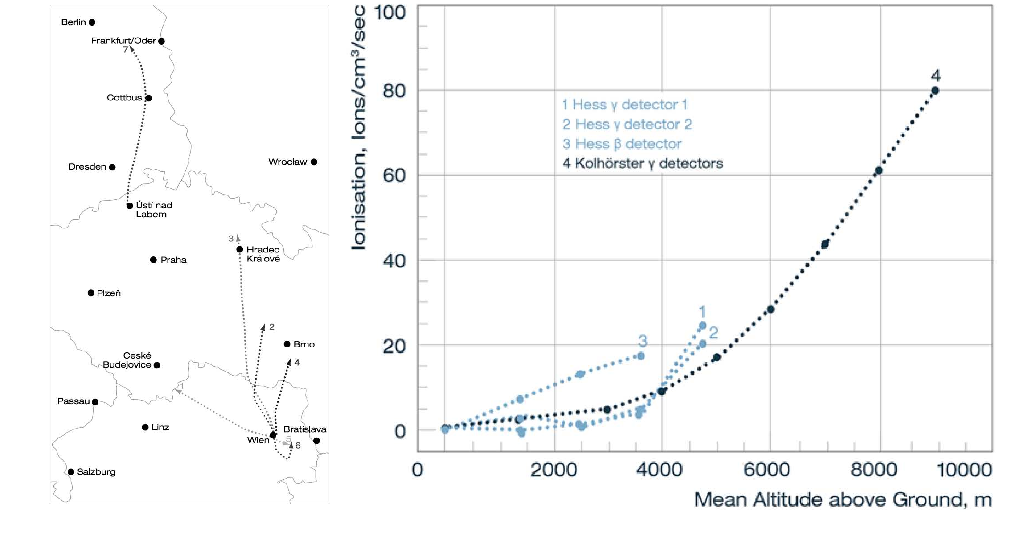
\includegraphics[width=0.88\hsize]{fig/hess-2018-fig3.pdf}
  \caption{Hess が 1912 年に実施した 7 回の気球飛行の経路（左）と、Hess の第 7 回飛行および Kolh\"orster の飛行で測定された電離率の高度依存（右）。右図では地上で測定された電離率が差し引かれている。De Angelis and Arcaro b. Schultz (2018) の Fig.~3 より引用~\cite{HessTranslation2018}。}
  \label{fig:hess_altitude}
\end{figure}

この透過性放射を宇宙起源の高周波電磁波と考えた Robert Andrews Millikan は、1925 年の \textit{Science} 論文で cosmic rays という名称を用いた~\cite{Millikan1925,Carlson2012}。

Jacob Clay は 1927 年に緯度効果を観測し、地磁気の影響を受ける荷電粒子が放射線に含まれることを示した。
1929 年、Walther Bothe と Werner Kolh\"orster は、上下に並べた 2 本の Geiger--M\"uller 計数管の間に厚さ \(4\ \mathrm{cm}\) の金板を置いた。金板を挿入しても同時計数率はわずかしか減少しなかった。この結果から、\(\gamma\) 線が物質中で作る Compton 電子ではなく、金板を通過する荷電粒子によって計数管が同時に作動したと結論した~\cite{Carlson2012}。
1933 年に観測された東西効果は、一次宇宙線の大部分が正電荷をもつことを示した。Marcel Schein らは 1940 年の気球実験で、陽子を主成分と同定した~\cite{Carlson2012}。これらの結果は Millikan の電磁波説を退けたが、cosmic rays という名称は残った。

Bruno Rossi は 1933 年、互いに離した計数管の同時計数が偶然同時計数の予測を上回ることから、広い範囲へ同時に到来する粒子群を初めて報告した~\cite{Rossi1933Showers}。
Pierre Auger、Roland Maze らは 1930 年代後半に検出器間の距離を数百メートルまで広げ、離れた検出器へ同時に到来する粒子群と、シャワー軸からの距離に対する粒子密度を測定した~\cite{Auger1939,Carlson2012}。
Rossi と Auger らの観測は、1 個の高エネルギー一次粒子から生じた多数の二次粒子が広範囲へ到来することを示し、空気シャワーによる間接観測の基礎となった。
John Linsley は Volcano Ranch 実験において、一次エネルギーが \(10^{20}\ \mathrm{eV}\) を超えると推定された空気シャワーを 1962 年に初めて観測し、翌年に報告した~\cite{Linsley1963,BluemerEngelHorandel2009}。
現在稼働する大規模観測施設のうち、Telescope Array（TA）と Pierre Auger Observatory は、地表検出器と大気蛍光望遠鏡を組み合わせ、エネルギー、質量組成、到来方向を相補的に測定している~\cite{PDGCosmicRays,AugerTA2023ArrivalDirections}。

\section{エネルギースペクトルと質量組成}
\subsection{エネルギースペクトル}\label{subsec:cosmic_ray_spectrum}
宇宙線のエネルギースペクトルは、単位エネルギー、面積、時間、立体角あたりの到来数を表す微分強度 \(J(E)\) で記述される。\(J(E)\) は広いエネルギー範囲でおおよそべき乗則
\begin{equation}
  J(E)
  \equiv
  \frac{\mathrm{d}N}{\mathrm{d}E\,\mathrm{d}A\,\mathrm{d}t\,\mathrm{d}\Omega}
  \propto E^{-\gamma}
\end{equation}
に従って減少する。ここでは正のスペクトル指数 \(\gamma\) を用い、その増加を軟化、減少を硬化と呼ぶ。ただし、単一のべき乗則で全エネルギー範囲を記述できるわけではない。図~\ref{fig:cosmic_ray_spectrum}に示すように、knee、second knee、ankle（くるぶし）、高エネルギー側のサプレッションといった折れ曲がりが見られる~\cite{PDGCosmicRays}。

\begin{figure}[htb]
  \centering
  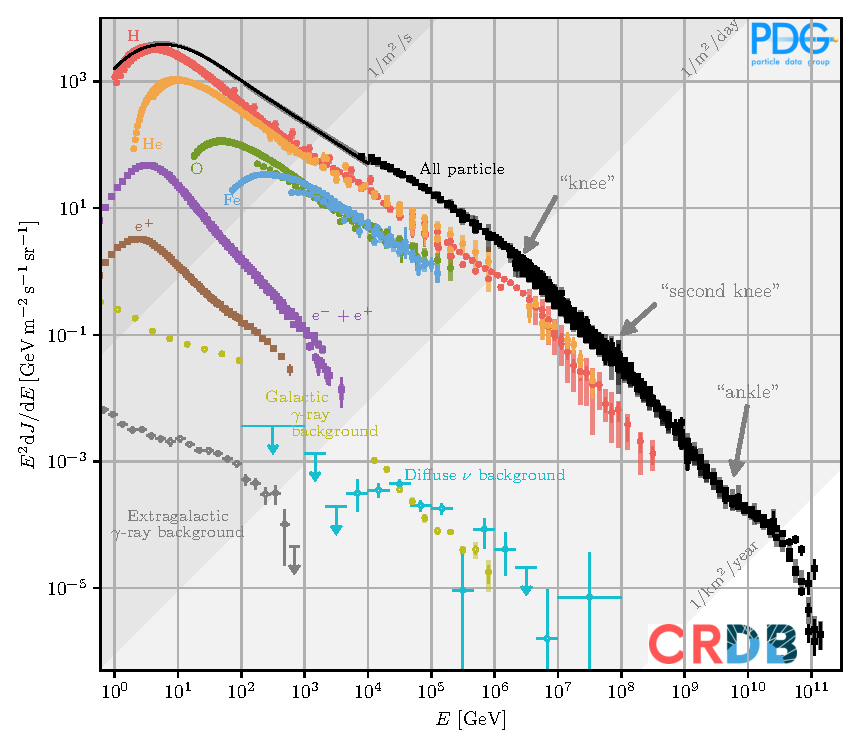
\includegraphics[width=0.85\hsize]{fig/Cosmic-Rays-Energy-Spectrum.pdf}
  \caption{宇宙線のエネルギースペクトル。PDG のレビュー \textit{Cosmic Rays} の Fig.~30.1 より引用~\cite{PDGCosmicRays}。}
  \label{fig:cosmic_ray_spectrum}
\end{figure}

低エネルギー側の宇宙線は、主として銀河系内起源と考えられる。同じ電荷の原子核では、エネルギーが高いほど銀河磁場で曲げられにくくなり、銀河系内に閉じ込められる時間も短くなる。ただし、銀河系外起源の寄与がどのエネルギーから卓越するかは確定していない。
スペクトルの折れ曲がりには、起源天体における加速限界、銀河系からの脱出、宇宙背景放射との相互作用などが関係する~\cite{PDGCosmicRays,Stanev2004}。

微分強度はエネルギーとともに急減する。そこで、折れ曲がりを見やすくするため、図の縦軸には \(J(E)\) にエネルギーの 3 乗を掛けた \(E^3J(E)\) を用いることが多い。
代表的な構造は、約 \(4\times10^{15}\ \mathrm{eV}\) の knee、\(10^{17}\ \mathrm{eV}\) から数 \(10^{17}\ \mathrm{eV}\) に報告される second knee、約 \(5\times10^{18}\ \mathrm{eV}\) の ankle、および約 \(5\times10^{19}\ \mathrm{eV}\) 以上のサプレッションである~\cite{PDGCosmicRays,LHAASOKnee2024,TALESpectrum2018,Horandel2003,AugerSpectrum2020}。
これらの名称は全粒子スペクトルの形状を表す観測的な用語であり、特定の物理機構をあらかじめ意味するものではない。
折れ曲がりの位置には、解析に用いる関数とエネルギースケールの不確かさが関係する。位置の自由な推定値と固定した値を区別し、統計誤差と系統誤差を分けて比較する必要がある~\cite{AugerTAEnergyScale2019,TALESpectrum2018}。Second knee の具体的な測定結果は第\ref{subsec:second_knee_observations}節にまとめる。

\subsection{質量組成}\label{subsec:cosmic_ray_composition}
質量組成は、エネルギースペクトルとは異なる観測量から、宇宙線の起源と伝搬を制約する。
質量数を \(A\)、同じエネルギーにおける核種 \(i\) の割合を \(f_i\) とすると、質量組成を表す量の一つとして
\begin{equation}
  \langle\ln A\rangle=\sum_i f_i\ln A_i,
  \qquad f_i\geq0,\qquad \sum_i f_i=1
  \label{eq:mean_lnA}
\end{equation}
を用いる。これは質量数の自然対数を核種の割合で平均した量であり、平均質量数の対数 \(\ln\langle A\rangle\) とは一般に異なる。陽子では \(\ln A=0\)、鉄では \(\ln A=\ln56\simeq4.03\) である。空気シャワーが最も発達する大気深さを \(X_{\max}\) といい、その分布から相互作用モデルを介して組成を推定する。
Fly's Eye は 1993 年、エネルギースペクトルの形が変わる領域で \(X_{\max}\) のエネルギー依存も変化することを報告した~\cite{FlysEyeComposition1993}。
その後、HiRes の大気蛍光望遠鏡と Michigan Muon Array（MIA）を組み合わせた HiRes--MIA 実験は、2001 年に同じ空気シャワーの \(X_{\max}\) と地表ミューオン密度を測定した~\cite{HiResMIA2001}。
Pierre Auger Observatory は 2014 年、\(10^{17.8}\ \mathrm{eV}\) 以上の \(X_{\max}\) 分布を測定し、平均と標準偏差の両方から質量組成を制約した~\cite{AugerXmax2014}。
TALE ハイブリッド検出器は \(10^{16.5}\)--\(10^{18.5}\ \mathrm{eV}\) の \(X_{\max}\) 分布を測定し、その平均のエネルギー依存に折れ曲がりを見いだした~\cite{TALEMassComposition2026}。この測定量と、核種ごとのモンテカルロシミュレーション（MC）の分布への適合から求める組成とは区別される。
図~\ref{fig:tale_hybrid_elongation}に示す平均 \(X_{\max}\) の折れ曲がりは、\(\log_{10}(E/\mathrm{eV})=17.13\pm0.04_{\mathrm{stat}}{}^{+0.05}_{-0.03}{}_{\mathrm{sys}}\) に得られている。その前後のエロンゲーションレートは、\(\log_{10}E\) の単位変化あたり \(23.3\pm5.6\) から \(97.6\pm4.5\ \mathrm{g\,cm^{-2}}\) へ増加する。ここで示した傾きの誤差は統計誤差であり、この変化から核種割合を求めるには相互作用モデルの予測が必要となる。

\begin{figure}[htb]
  \centering
  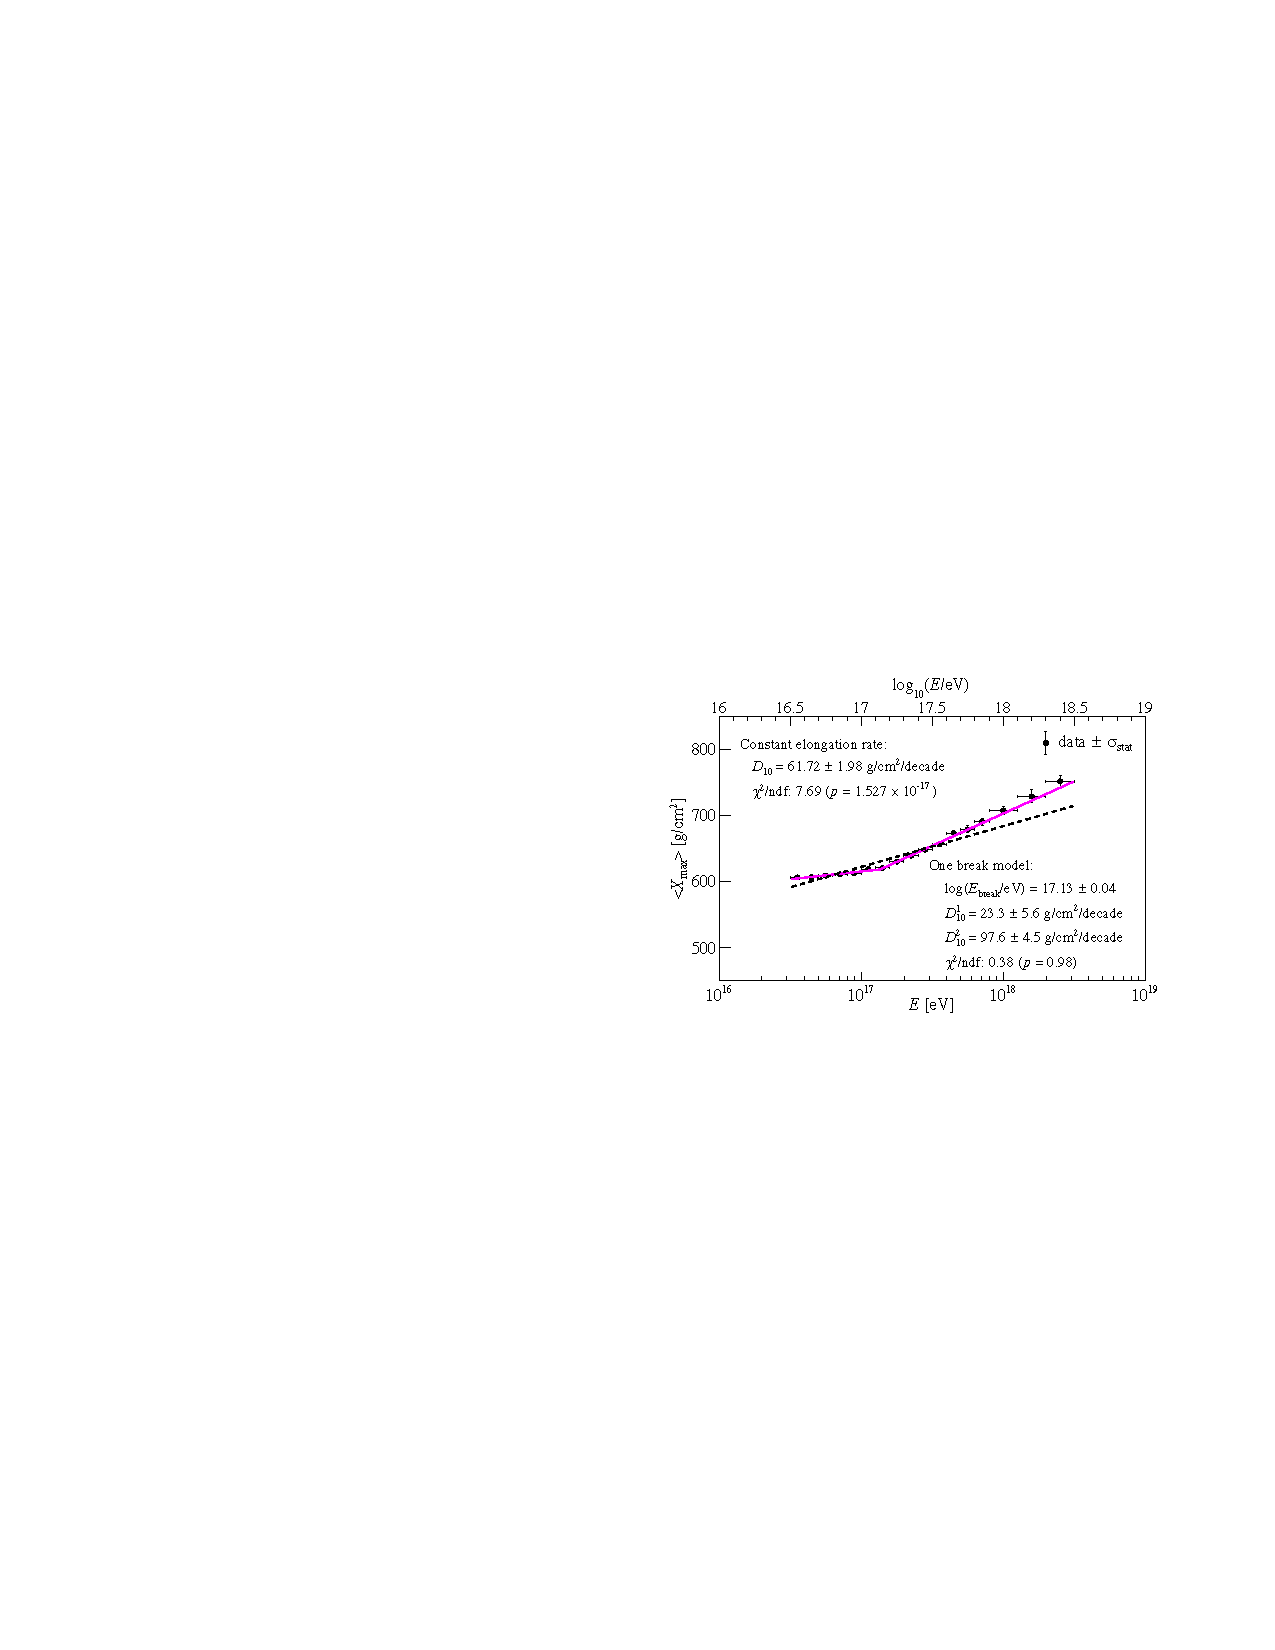
\includegraphics[width=0.68\hsize]{fig/tale-hybrid-2026-fig14.pdf}
  \caption{TALE Hybrid による平均 \(X_{\max}\) のエネルギー依存。点と誤差棒は測定値と統計誤差、破線は単一のエロンゲーションレート、マゼンタ線は折れ曲がりをもつ直線のフィットを示す。全粒子スペクトルの折れ曲がりとは異なる測定量である。R. U. Abbasi et al., ``Cosmic ray mass composition measurement in the energy range from \(10^{16.5}\) eV to \(10^{18.5}\) eV observed with the TALE hybrid detector'', Phys. Rev. D 113, 062003 (2026), DOI:10.1103/vrky-dxn7, Fig.~14（arXiv:2603.14804v1）より転載~\cite{TALEMassComposition2026}。\href{https://creativecommons.org/licenses/by/4.0/}{CC BY 4.0}。図の内容は変更していない。}
  \label{fig:tale_hybrid_elongation}
\end{figure}

図~\ref{fig:tale_lna}は、同じ解析から推定された \(\langle\ln A\rangle\) を他実験と比較している。平均的に組成が軽くなり始めることは、重い成分が消失したことや、銀河系外成分が優勢になったことを、それだけで意味するわけではない。

\begin{figure}[htb]
  \centering
  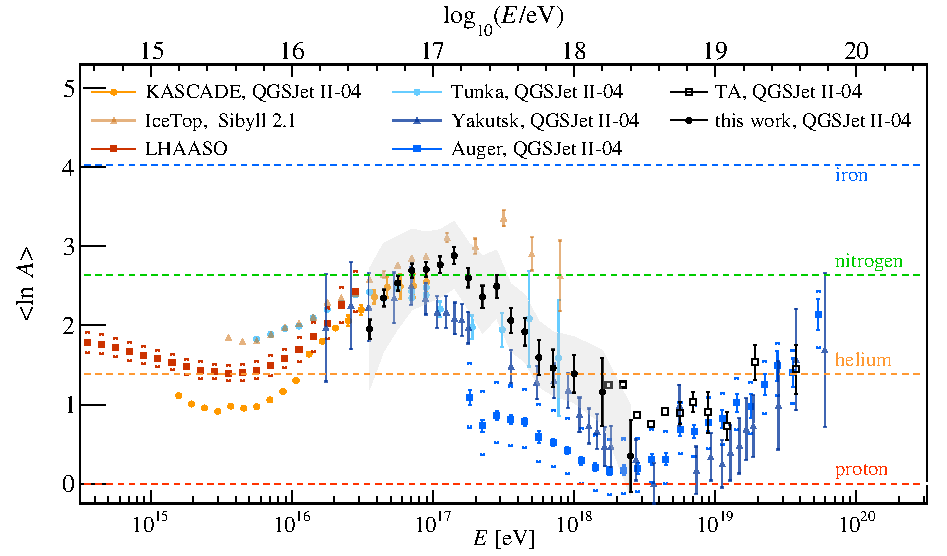
\includegraphics[width=0.85\hsize]{fig/TALE-Hybrid-lnA.pdf}
  \caption{各実験で推定された \(\langle\ln A\rangle\) の比較。黒丸は TALE ハイブリッド解析の結果で、QGSJetII-04 に基づく核種割合から求めている。灰色帯は同解析の系統的不確かさを表す。他実験に用いたハドロン相互作用モデルは凡例に記されており、同一モデルで統一した比較ではない。TALE ハイブリッド質量組成測定の Fig.~22 より引用~\cite{TALEMassComposition2026}。}
  \label{fig:tale_lna}
\end{figure}

質量組成は、エネルギースペクトルの折れ曲がりの解釈と密接に関係する。各核種の最大エネルギーが電荷 \(Z\) に比例する場合、陽子のスペクトルが先に急減し、電荷の大きい原子核はより高いエネルギーまで残る。このとき、knee から second knee にかけて重い原子核の割合が増える。
一方、銀河系外起源の陽子やヘリウム原子核が加われば、軽い原子核の割合と平均 \(X_{\max}\) が増加する。全粒子強度 \(J(E)\)、電荷群別スペクトル、\(\langle X_{\max}\rangle\)、\(\sigma(X_{\max})\)、ミューオン数、到来方向分布は、こうした起源成分の変化を異なる側面から制約する~\cite{PDGCosmicRays,TALEMassComposition2026}。

\section{観測手法と主要実験}\label{subsec:cosmic_ray_experiments}
一次宇宙線を検出器で捉える直接観測では、磁気スペクトロメータやカロリメータによって粒子の電荷とエネルギーを測定できる。
衛星・気球実験である AMS-02、CREAM、DAMPE、CALET などは、GeV からサブ PeV 領域における核種別のエネルギースペクトルを高精度で測定している~\cite{AMSProton2015,CREAM2011,DAMPEProton2019,CALETProton2022}。
直接観測では核種を個別に識別できる一方、検出器の受容面積と飛翔時間が限られるため、強度が急減する PeV 以上では十分な統計量を得にくい。

間接観測では、一次宇宙線が大気中に作る空気シャワーを測定する。地表アレイは、検出器に入射する粒子の信号と到来時刻を高い稼働率で記録する。信号に含まれる電磁成分とミューオン成分の割合は、検出器の材質、観測高度、天頂角、シャワー軸からの距離によって異なる。
光学観測にも複数の方法がある。結像型の望遠鏡は蛍光やチェレンコフ光の像と時間変化から縦方向発達を再構成する。TALE ではチェレンコフ光を多く含む事象も利用する。一方、Tunka-133 は地表に配置した非結像型の光検出器でチェレンコフ光の密度と時間情報を測る~\cite{TALESpectrum2018,TALEMassComposition2026,TunkaSpectrum2020}。蛍光観測は大気へのエネルギー付与をほぼカロリメトリックに測れるが、空の明るさや気象条件に制約され、地表観測より稼働率が低い。運用条件は装置と解析ごとに定められる。
電波観測は、地磁気効果と Askaryan 効果による MHz 帯の電波放射を利用する方法である~\cite{PDGCosmicRays}。検出器、観測量、エネルギーへの換算を区別して、代表的な実験を表~\ref{tab:cosmic_ray_experiments}に示す。較正方法の詳細は第\ref{sec:energy_calibration}節で述べる。

\begin{table}[htb]
  \centering
  \small
  \caption{Knee から超高エネルギー領域を測定する代表的な実験の検出器、主要な観測量、エネルギー換算。観測量の選択と較正範囲は各解析に依存する。}
  \label{tab:cosmic_ray_experiments}
  \begin{tabular}{@{}p{0.16\hsize}p{0.22\hsize}p{0.24\hsize}p{0.25\hsize}@{}}
    \hline
    実験 & 検出器 & 主要な観測量 & エネルギー換算・較正 \\
    \hline
    KASCADE-Grande & シンチレータとミューオン検出器 & 荷電粒子数 \(N_{\mathrm{ch}}\) とミューオン数 \(N_\mu\) & 両観測量と MC の関係を用いる~\cite{KASCADEGrandeHeavyKnee2011} \\
    LHAASO & 地表粒子・ミューオン検出器と広視野チェレンコフ望遠鏡など & 粒子数、ミューオン数、チェレンコフ像 & 検出器の組合せごとに MC と較正を用いる~\cite{LHAASOKnee2024,LHAASOProton2025} \\
    IceTop/IceCube & 氷上タンクと氷中光検出器 & 電磁・ミューオン成分を含む地表信号と氷中ミューオン束 & MC に基づきスペクトルと組成を再構成する~\cite{IceTopComposition2019} \\
    Tunka-133 & 非結像型チェレンコフ光検出器 & 光密度 \(Q(200)\) と光パルスの時間情報 & MC の換算関係と QUEST に基づく規格化を用いる~\cite{TunkaSpectrum2020} \\
    TALE & 蛍光・チェレンコフ望遠鏡と地表シンチレータ & 光量と縦方向発達、地表信号、到来時刻 & 光学解析では縦発達の積分と不可視エネルギー補正を用いる~\cite{TALESpectrum2018,TALEMassComposition2026} \\
    Pierre Auger & 水チェレンコフ地表検出器と蛍光望遠鏡 & 地表信号と蛍光によるエネルギー付与 & 天頂角補正後の信号を FD 尺度へ較正する~\cite{AugerSecondKnee2021} \\
    \hline
  \end{tabular}
\end{table}
\FloatBarrier

地表アレイと光学検出器は、粒子密度、到来時刻、光量、縦方向発達などを測定し、そこから一次粒子のエネルギーと質量を再構成する。
エネルギーの再構成には、大気状態、検出器の較正、不可視エネルギーの補正が関係する。質量の推定結果は、シミュレーションに用いるハドロン相互作用モデルによっても変化する。
検出原理や観測高度の異なる実験の比較は、測定法に固有の系統差と、複数の測定法に共通するモデル依存性を分けて評価する手掛かりとなる。

\section{非熱的粒子加速}\label{subsec:acceleration_need}\label{subsec:fermi_acceleration}
宇宙線の加速天体と加速機構は、エネルギースペクトルや質量組成を解釈するうえで中心的な問題である。
熱的な粒子分布だけでは PeV から EeV 領域の粒子を説明できない。
たとえば \(10^{15}\ \mathrm{eV}\) の陽子は、温度に換算すれば \(10^{19}\ \mathrm{K}\) 以上に対応するため、通常の熱平衡プラズマからそのまま出てくる粒子とは考えにくい。
このエネルギー領域の宇宙線は、天体プラズマの磁場中で散乱を繰り返しながらエネルギーを得る非熱的過程によって生成される。

衝撃波などの加速領域で作られる源スペクトルは、銀河磁場中の拡散、エネルギー損失、相互作用、脱出を経て変形する。
地球で測定されるスペクトル指数は加速と伝搬の双方に依存するため、加速源における値とは一致しない~\cite{Gabici2019,PDGCosmicRays}。

Enrico Fermi は 1949 年、運動する磁気雲との確率的相互作用による 2 次加速を提案した~\cite{Fermi1949}。
1 次フェルミ加速に相当する拡散衝撃波加速は、Bell と Blandford--Ostriker らによって 1970 年代末に独立に定式化された~\cite{Bell1978,BlandfordOstriker1978,Drury1983}。
両者に共通する基本は、荷電粒子が運動する磁場構造と何度も相互作用し、そのたびに少しずつエネルギーを変えることである。
ここでいう磁場構造とは、乱流磁場、磁化した雲、衝撃波の上流・下流にある磁気不規則性などである。
理想磁気流体近似を適用した局所プラズマ静止系では、電場がほぼ消える。そのため、粒子は磁場で向きを変えるだけであり、散乱自体によるエネルギー損失はない。
散乱体は観測者に対して運動しており、散乱の前後には異なる慣性系へのローレンツ変換が入る。このため、観測者の系では粒子エネルギーが変化する。

\subsection{散乱体との 1 回の相互作用}
散乱体が \(x\) 方向に速度 \(u\) で動いているとする。
\(\beta_u=u/c\)、ローレンツ因子 \(\Gamma_u=(1-\beta_u^2)^{-1/2}\) と定義し、粒子は相対論的で \(v\simeq c\) とする。
散乱前の粒子エネルギーを観測者系で \(E_1\)、粒子方向と散乱体速度のなす角を \(\theta_1\) とし、\(\mu_1=\cos\theta_1\) とおく。
このとき、散乱体静止系で見た粒子エネルギーは
\begin{equation}
  E_1'
  =
  \Gamma_u E_1(1-\beta_u\mu_1)
\end{equation}
である。
散乱体静止系で散乱が弾性的なら \(E_2'=E_1'\) である。
散乱体静止系における散乱後の粒子方向と \(x\) 軸のなす角を \(\theta_2'\) とし、\(\mu_2'=\cos\theta_2'\) とすると、観測者系に戻したエネルギーは
\begin{equation}
  E_2
  =
  \Gamma_u E_2'(1+\beta_u\mu_2')
  =
  \Gamma_u^2 E_1(1-\beta_u\mu_1)(1+\beta_u\mu_2')
  \label{eq:fermi_energy_transform}
\end{equation}
となる。
\(\beta_u\ll1\) で展開すると
\begin{equation}
  \frac{\Delta E}{E_1}
  \equiv
  \frac{E_2-E_1}{E_1}
  \simeq
  \beta_u(\mu_2'-\mu_1)
  +
  \beta_u^2(1-\mu_1\mu_2')
\end{equation}
である。
したがって、散乱体へ正面から近づく粒子では \(\theta_1>\pi/2\)、すなわち \(\mu_1<0\) となり、平均的にエネルギーを得やすい。
逆に、散乱体へ後ろから追いつく粒子はエネルギーを失いやすい。

\subsection{2 次フェルミ加速}
乱流中の磁化した雲のように、散乱体がいろいろな方向へほぼ等方的に動いている場合を考える。
粒子の入射方向が等方的でも、衝突頻度は相対速度に比例するため、\(\mu_1=\cos\theta_1\) で表した入射方向に対する散乱確率は \(1-\beta_u\mu_1\) に比例する。
この重みを付けて平均すると
\begin{equation}
  \langle\mu_1\rangle
  =
  \frac{\int_{-1}^{1}\mu(1-\beta_u\mu)\,\mathrm{d}\mu}
       {\int_{-1}^{1}(1-\beta_u\mu)\,\mathrm{d}\mu}
  =
  -\frac{\beta_u}{3}
\end{equation}
となる。
一方、散乱体静止系で散乱後の方向が等方化されるなら \(\langle\mu_2'\rangle=0\) である。
式~\eqref{eq:fermi_energy_transform}の展開式を平均すると
\begin{equation}
  \left\langle\frac{\Delta E}{E}\right\rangle
  \simeq
  \frac{4}{3}\beta_u^2
  =
  \frac{4}{3}
  \left(\frac{u}{c}\right)^2
\end{equation}
を得る。
これが 2 次フェルミ加速である。
平均的なエネルギー増加が散乱体速度の 2 乗に比例するため、2 次フェルミ加速は乱流中の再加速に寄与する一方、単独で宇宙線を最高エネルギーまで短時間で加速する機構としては効率が低い。

\subsection{1 次フェルミ加速}
衝撃波静止系では、上流のプラズマは衝撃波へ流入し、下流のプラズマは衝撃波から流れ去る。両者は同じ向きに流れるが、その速さは \(u_1>u_2>0\) を満たす。
粒子は上流と下流の磁気不規則性で散乱されながら衝撃波面を何度も横切り、各側のプラズマ静止系ではほぼ等方化される。
衝撃波静止系で上流速度を \(u_1\)、下流速度を \(u_2\) とし、圧縮比を
\begin{equation}
  r=\frac{u_1}{u_2}
\end{equation}
と定義する。
衝撃波を横切るプラズマには非相対論的近似 \(u_1,u_2\ll c\) を適用するが、加速される粒子は相対論的であるとする。
この近似では、上流と下流の相対速度を \(u_1-u_2\) と書け、エネルギー変化は \(u_i/c\) の 1 次までで扱える。
粒子速度は \(v\simeq c\) と置き、衝撃波を横切る粒子フラックスとエネルギー変化を評価する。

テスト粒子（test-particle）近似とは、加速された宇宙線の圧力が衝撃波構造を変えるほど大きくないとみなす近似である。
この近似では、上流・下流の流速や圧縮比 \(r\) は通常の流体力学的な Rankine--Hugoniot 関係で決まる。宇宙線の反作用による衝撃波前駆領域やスペクトルの曲がりは考慮しない。
この仮定から得られるスペクトル指数は、非線形な衝撃波加速ではなく、最も単純な拡散衝撃波加速に対応する~\cite{Drury1983}。

粒子分布のほぼ等方性は、上流・下流それぞれのプラズマ静止系で磁気不規則性による散乱が十分頻繁に起こる、という仮定である。
この仮定により、粒子は衝撃波を何度も横切り、上流から下流、下流から上流への各横断を統計的に平均できる。
また、等方分布の粒子が片側から面を横切る粒子フラックスは
\begin{equation}
  \int_0^1 n c\,\mu\,\frac{\mathrm{d}\mu}{2}
  =
  \frac{nc}{4}
\end{equation}
となる。
ここで \(\mu\) は、粒子の進行方向と面法線のなす角 \(\theta\) に対して \(\mu=\cos\theta\) とおいた量である。
この \(nc/4\) は、後述する加速領域からの逃走確率の見積もりに用いる。

衝撃波を横切る粒子の角度分布を粒子フラックスで重み付けすると、\(\mu\) の平均は
\begin{equation}
  \langle\mu\rangle_{\mathrm{cross}}
  =
  \frac{\int_0^1 \mu^2\,\mathrm{d}\mu}
       {\int_0^1 \mu\,\mathrm{d}\mu}
  =
  \frac{2}{3}
\end{equation}
となる。
このため、片道の平均エネルギー増加はおおよそ
\begin{equation}
  \left\langle\frac{\Delta E}{E}\right\rangle_{\mathrm{one\ crossing}}
  \simeq
  \frac{2}{3}\frac{u_1-u_2}{c}
\end{equation}
である。
粒子は上流から下流へ、さらに下流から上流へ戻ることで 1 サイクルを作るので、1 サイクルあたりの平均的なエネルギー増加率は
\begin{equation}
  \xi
  \equiv
  \left\langle\frac{\Delta E}{E}\right\rangle_{\mathrm{cycle}}
  \simeq
  \frac{4}{3}
  \frac{u_1-u_2}{c}
\end{equation}
となる。
これは速度の 1 次に比例するため、1 次フェルミ加速と呼ばれる。

衝撃波加速でべき乗スペクトルが生じるのは、エネルギー増加と逃走が競合するためである。
下流側の粒子分布を等方的とすると、単位面積あたりに衝撃波へ戻る粒子フラックスは、上記のとおり \(nc/4\) である。
一方、下流プラズマは速度 \(u_2\) で粒子を衝撃波から遠ざけるので、移流による損失フラックスは \(nu_2\) である。
したがって、1 サイクルごとに粒子が加速領域から逃げる確率は
\begin{equation}
  P_{\mathrm{esc}}
  \simeq
  \frac{nu_2}{nc/4}
  =
  \frac{4u_2}{c}
\end{equation}
と見積もられる。
\(k\) 回のサイクル後には
\begin{equation}
  E_k=E_0(1+\xi)^k,
  \qquad
  N_k=N_0(1-P_{\mathrm{esc}})^k
\end{equation}
である。
したがって
\begin{align}
  N(>E)
  &\propto
  \left(\frac{E}{E_0}\right)^{
  \ln(1-P_{\mathrm{esc}})/\ln(1+\xi)}
  \\
  &\simeq
  \left(\frac{E}{E_0}\right)^{-P_{\mathrm{esc}}/\xi}
\end{align}
となる。
この積分スペクトルを微分スペクトルに直すと
\begin{equation}
  \frac{\mathrm{d}N}{\mathrm{d}E}
  \propto
  E^{-s},
  \qquad
  s
  =
  1+\frac{P_{\mathrm{esc}}}{\xi}
  =
  \frac{r+2}{r-1}
\end{equation}
である~\cite{BlandfordOstriker1978,Drury1983}。
強い非相対論的衝撃波では、断熱指数 \(5/3\) の気体に対して \(r\simeq4\) となるため、\(s\simeq2\) が得られる。
これは加速源のスペクトルを表す。地球で観測されるスペクトルは、銀河内拡散やエネルギー依存の脱出によってさらに変化する。

\subsection{源スペクトルから観測スペクトルへの変化}
観測されるべき乗則は、加速領域で作られる源スペクトルと伝搬中の変化によって決まる。
単一核種を対象とし、連続的なエネルギー損失、核破砕、二次粒子生成を省いた leaky-box 型モデルを考える。単位体積・単位エネルギー当たりの粒子数を \(n(E)\)、単位時間当たりの注入率を \(Q(E)\)、銀河からの脱出時間を \(\tau_{\mathrm{esc}}(E)\) とすると、輸送方程式は
\begin{equation}
  \frac{\partial n}{\partial t}
  =Q(E)-\frac{n(E)}{\tau_{\mathrm{esc}}(E)}
  \label{eq:leaky_box}
\end{equation}
と書ける。
定常状態では
\begin{equation}
  n(E)=Q(E)\tau_{\mathrm{esc}}(E)
\end{equation}
である。
運動量を \(p\)、核電荷を \(Ze\)、光速を \(c\) とし、リジディティを \(\mathcal R=pc/(Ze)\) と定義する。\(e\) は電気素量であり、リジディティは電位の次元をもつ。注入スペクトルを \(Q(E)\propto E^{-s}\)、拡散係数を \(D(\mathcal{R})\propto\mathcal{R}^{\delta}\) とする。
銀河ハローの代表的な高さを \(H\) とすれば、拡散脱出時間は
\begin{equation}
  \tau_{\mathrm{esc}}
  \sim \frac{H^2}{D(\mathcal{R})}
  \propto \mathcal{R}^{-\delta}
\end{equation}
である。
単一の核種について相対論的極限 \(E\propto\mathcal{R}\) を考えると、地球で観測される強度は
\begin{equation}
  J(E)\propto n(E)\propto E^{-(s+\delta)}
  \label{eq:source_propagation_spectrum}
\end{equation}
となる~\cite{Strong2007,Gabici2019}。
したがって、強い衝撃波による \(s\simeq2\) の源スペクトルに、\(\delta>0\) のエネルギー依存脱出を加えると、地球ではより急なスペクトルが観測される。
実際には、拡散係数の空間依存、移流、再加速、核破砕、離散的な宇宙線源が寄与するため、式~\eqref{eq:leaky_box}は完全な銀河伝搬モデルではない。
それでも、加速領域では一定割合の利得と一定確率の逃走が繰り返され、銀河内伝搬では滞在時間がリジディティに依存する。式~\eqref{eq:source_propagation_spectrum}は、これら 2 つのスケール不変過程から広いエネルギー範囲にべき乗則が現れることを端的に示している。
スペクトルの折れ曲がりは、この近似的なスケール不変性が加速限界、伝搬過程の変化、または異なる起源成分の重なりによって破れるエネルギー領域と解釈できる。

\section{リジディティと宇宙線の閉じ込め}
拡散衝撃波加速から得たスペクトル指数は、「加速される粒子が十分な回数だけ衝撃波を往復できる」という仮定に基づく。
実際にどこまで高いエネルギーに到達できるかは、加速時間と損失時間・脱出時間の競合で決まる。
拡散係数を上流・下流でそれぞれ \(\kappa_1\)、\(\kappa_2\) とすると、非相対論的な拡散衝撃波加速の代表的な加速時間は
\begin{equation}
  t_{\mathrm{acc}}
  \simeq
  \frac{3}{u_1-u_2}
  \left(
    \frac{\kappa_1}{u_1}
    +
    \frac{\kappa_2}{u_2}
  \right)
\end{equation}
と書ける~\cite{Drury1983}。
到達可能エネルギーは、磁場の強さ、乱流による散乱効率、加速領域の大きさ、天体の寿命、放射損失、相互作用損失によって制限される。

\subsection{リジディティとラーモア半径}\label{subsec:rigidity_larmor}
磁場中の宇宙線の運動は、エネルギー \(E\) と電荷 \(Ze\) の双方に依存する。
同じエネルギーでも、陽子と鉄原子核では磁場中の曲がり方が異なる。
同じ磁場中で荷電粒子がどれだけ曲げられにくいかを表す量が、リジディティ（rigidity）
\begin{equation}
  \mathcal{R}=\frac{pc}{Ze}
\end{equation}
である。
ここで \(p\) は運動量である。
高エネルギーでは \(E\simeq pc\simeq Ze\mathcal R\) である。\(E\) を eV、\(\mathcal R\) を V で表した数値の関係は \(E[\mathrm{eV}]\simeq Z\mathcal R[\mathrm V]\) となる。同じ \(E\) なら \(Z\) の大きい原子核ほど \(\mathcal{R}\) は小さく、磁場で曲げられやすい。

一様磁場中で、磁場に垂直な運動量成分を \(p_{\perp}\) とする。
以下の磁場を含む式にはガウス単位系を用いる。この単位系ではローレンツ力は \((Ze/c)\boldsymbol{v}\times\boldsymbol{B}\) であり、円運動の向心力条件は
\begin{equation}
  \frac{Ze}{c}v_{\perp}B
  =
  \frac{p_{\perp}v_{\perp}}{r_{\mathrm{L}}}
\end{equation}
である。
ここからラーモア半径
\begin{equation}
  r_{\mathrm{L}}
  =
  \frac{p_{\perp}c}{ZeB}
\end{equation}
が得られる。
閉じ込め条件のような桁の見積もりでは \(p_{\perp}\sim p\) と置き、相対論的粒子では \(E\simeq pc\) を用いるため、
\begin{equation}
  r_{\mathrm{L}}
  \simeq
  \frac{pc}{ZeB}
  \simeq
  \frac{E}{ZeB}
  \label{eq:larmor_radius}
\end{equation}
となる。
数値的には
\begin{equation}
  r_{\mathrm{L}}
  \simeq
  1.08\ \mathrm{kpc}
  \left(\frac{E}{1\ \mathrm{EeV}}\right)
  \left(\frac{Z}{1}\right)^{-1}
  \left(\frac{B}{1\ \mu\mathrm{G}}\right)^{-1}
\end{equation}
である。
この式によれば、\(1\ \mu\mathrm{G}\) の磁場中にある \(1\ \mathrm{EeV}\) 陽子のラーモア半径は kpc 程度である。
一方、同じエネルギーの鉄原子核では半径は約 \(1/26\) になる。
この \(Z\) 依存性が、knee 付近の構造や最高エネルギーでの質量組成を議論するときの基礎になる~\cite{PDGCosmicRays,Gabici2019}。

\subsection{閉じ込め条件と Hillas 図}\label{subsec:hillas_condition}
粒子の加速には、加速領域内への閉じ込めが必要である。
加速領域の代表的な大きさを \(L\)、磁場を \(B\) とすると、閉じ込めの必要条件は
\begin{equation}
  r_{\mathrm{L}}\lesssim L
\end{equation}
である。
式~\eqref{eq:larmor_radius}を代入すると、閉じ込めだけから
\begin{equation}
  E_{\max}
  \lesssim
  ZeBL
\end{equation}
が得られる。
さらに、加速は無限に速く起こるわけではない。
加速領域内の流れや衝撃波の速度を \(v=\beta c\) とし、加速時間を
\begin{equation}
  t_{\mathrm{acc}}
  \sim
  \eta
  \frac{r_{\mathrm{L}}}{\beta^2 c}
\end{equation}
と見積もる。
ここで \(\eta\geq1\) は拡散係数や散乱効率を表す係数であり、Bohm 拡散の極限に近いほど小さい。
一方、粒子が加速領域に滞在できる時間はおおよそ
\begin{equation}
  t_{\mathrm{dyn}}
  \sim
  \frac{L}{\beta c}
\end{equation}
である。
\(t_{\mathrm{acc}}\lesssim t_{\mathrm{dyn}}\) を課すと
\begin{equation}
  E_{\max}
  \lesssim
  \frac{ZeBL\beta}{\eta}
\end{equation}
となる。
Hillas 図では、\(\eta\sim1\) とした楽観的な必要条件を
\begin{equation}
  E_{\max}\lesssim ZeBL\beta
  \label{eq:hillas_condition}
\end{equation}
と書く~\cite{Hillas1984,KoteraOlinto2011}。
数値的には
\begin{equation}
  E_{\max}
  \lesssim
  0.9\ Z\beta
  \left(\frac{B}{1\ \mu\mathrm{G}}\right)
  \left(\frac{L}{1\ \mathrm{kpc}}\right)
  \mathrm{EeV}
\end{equation}
である。
宇宙線の最大エネルギーは、磁場強度、加速領域の大きさ、速度、粒子の電荷によって制限される。
ただし Hillas 条件は必要条件であって十分条件ではない。
起源天体の候補は、Hillas 条件に加えて、天体の寿命に対する加速時間、シンクロトロン放射や光核反応による損失、粒子の脱出、および到来方向・質量組成との整合性によって制限される~\cite{KoteraOlinto2011,GlobusBlandford2023}。

図~\ref{fig:hillas_plot}は、代表的な候補天体の大きさと磁場強度を 2 軸に取り、式~\eqref{eq:hillas_condition}に対応する必要条件を示す Hillas 図である。図中の横軸 \(R\) は本稿の \(L\) に相当する。
一定の電荷と \(\beta\) に対するエネルギーの上限を示す \(BL=\mathrm{const.}\) の線は、両軸を対数で表すと傾き \(-1\) の直線になる。特定のエネルギーの陽子についてこの必要条件を満たす候補天体は、その直線より \(BL\) の大きい側に分布する。
鉄原子核では \(Z=26\) であるため、同じ \(B\) と \(L\) に対する閉じ込めの上限は陽子の約 26 倍になる。ただし、この図が示すのは閉じ込めの必要条件であり、実際の最大エネルギーは加速時間やエネルギー損失によっても制限される。

\begin{figure}[htb]
  \centering
  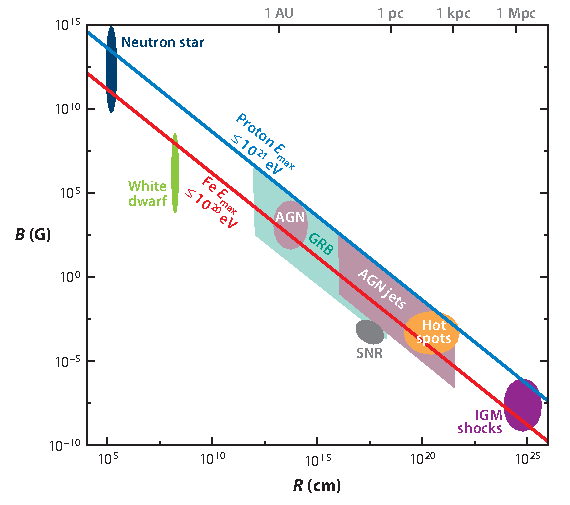
\includegraphics[width=0.85\hsize]{fig/Hillas-plot.pdf}
  \caption{候補天体の大きさと磁場強度を比較した Hillas 図。Kotera and Olinto (2011) の Fig.~8 より引用~\cite{KoteraOlinto2011}。}
  \label{fig:hillas_plot}
\end{figure}
\FloatBarrier

\section{Knee から second knee に至る核種別スペクトル}\label{subsec:knee_observations}
\subsection{全粒子 knee の測定}
Kulikov と Khristiansen は 1958 年、Moscow State University における測定で宇宙線スペクトルの knee を初めて報告した~\cite{KulikovKhristiansen1959,Horandel2003}。
彼らは、空気シャワーの電磁成分から求めたサイズ分布に折れ曲がりを見いだした。
英訳論文は 1959 年に刊行されており、\(10^6\)--\(10^7\) 個の粒子を含むシャワーの領域でサイズ分布の傾きが変化する可能性を論じている~\cite{KulikovKhristiansen1959}。
この観測は一次宇宙線のエネルギースペクトルを核種別に測ったものではなく、電磁成分から求めたシャワーサイズ分布の折れ曲がりであった。
その後、Akeno は電子数とミューオン数から独立に再構成したスペクトルが整合することを示し、\(10^{15.67}\ \mathrm{eV}\) 付近でスペクトル指数が約 2.62 から 3.02 へ変化すると報告した~\cite{AkenoSpectrum1984}。
さらに、異なるシャワー成分を利用し、異なる高度で行われた測定でも類似の急峻化が確認された。これらの一致は、knee が単一検出器の応答変化ではなく、一次宇宙線スペクトルに由来する構造であることを裏付けた~\cite{KASCADEDetector2003,PDGCosmicRays}。

LHAASO-KM2A は 2024 年、\(0.3\)--\(30\ \mathrm{PeV}\) の全粒子スペクトルと \(\langle\ln A\rangle\) を同時に測定した。
折れ曲がりエネルギーは
\begin{equation}
  E_k=3.67\pm0.05_{\mathrm{stat}}\pm0.15_{\mathrm{sys}}\ \mathrm{PeV}
\end{equation}
であり、スペクトル指数はその前後で \(2.7413\) から \(3.128\) へ増加した~\cite{LHAASOKnee2024}。
同解析では \(\langle\ln A\rangle\) が \(0.3\ \mathrm{PeV}\) から約 \(3\ \mathrm{PeV}\) まで減少し、knee より上で増加へ転じた。
この結果は、全粒子 knee におけるスペクトルの急峻化と、陽子など軽い原子核の減少が関係することを示す。ただし、\(\langle\ln A\rangle\) は平均量であるため、knee を作る核種と個々のスペクトルはこの測定だけでは決まらない。
図~\ref{fig:lhaaso_knee_mass}では、全粒子スペクトルの急峻化と \(\langle\ln A\rangle\) の増加への転換が、同じエネルギー領域に現れている。

\begin{figure}[htb]
  \centering
  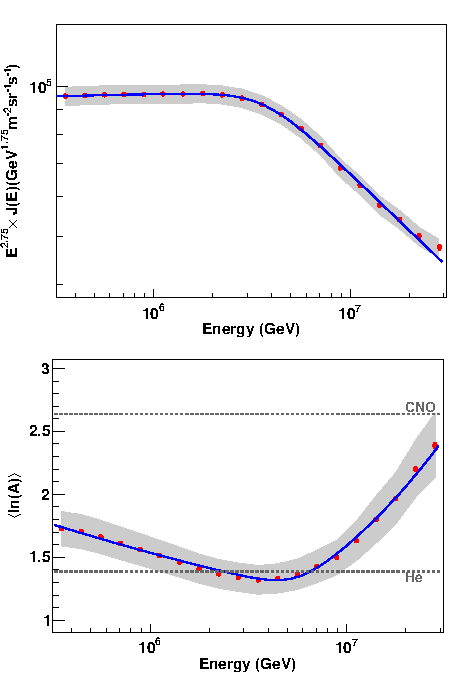
\includegraphics[width=0.56\hsize]{fig/lhaaso-knee-2024-fig3.pdf}
  \caption{LHAASO-KM2A が測定した全粒子エネルギースペクトル（上）と \(\langle\ln A\rangle\)（下）。灰色帯は系統的不確かさ、青線は折れ曲がりを含む適合結果を表す。LHAASO Collaboration (2024) の Fig.~3 より引用~\cite{LHAASOKnee2024}。}
  \label{fig:lhaaso_knee_mass}
\end{figure}

\subsection{陽子・ヘリウム成分と陽子スペクトル}
EAS-TOP は電磁成分とミューオン成分の相関から、knee 付近で重い原子核の割合が増えることを示した。また、ヘリウムのスペクトルが \((3.5\pm0.3)\ \mathrm{PeV}\) 付近で折れ曲がり、全粒子 knee に寄与する可能性を報告した~\cite{EASTOPComposition2004}。
KASCADE は電子数とミューオン数の二次元分布を使い、5 つの質量群に分けてスペクトルを再構成した。その結果、全粒子 knee は主として軽い原子核の減少に由来すると示された~\cite{KASCADEComposition2005}。
ただし、各質量群の絶対強度と折れ曲がりのエネルギーは、シミュレーションに QGSJET と SIBYLL のどちらを用いるかによって異なった。

ARGO-YBJ と LHAASO 広視野チェレンコフ望遠鏡の試作機によるハイブリッド観測は、陽子とヘリウムを合わせたスペクトルが \(0.7\ \mathrm{PeV}\) 付近で急峻化することを 2015 年に報告した~\cite{ARGOYBJLHAASOLightKnee2015}。
この測定では、陽子・ヘリウム成分の折れ曲がりが全粒子 knee より低いエネルギーに現れた。この結果は、同成分が数 PeV まで続くとしたほかの解析とは一致しなかった。
陽子を選別した GRAPES-3 の測定は、\(50\ \mathrm{TeV}\)--\(1.3\ \mathrm{PeV}\) のミューオン多重度分布に基づき、\(166\ \mathrm{TeV}\) 付近でスペクトルの傾きが有意に緩やかになることを示した~\cite{GRAPES3Proton2024}。
この測定の上限は \(1.3\ \mathrm{PeV}\) であり、数 \(\mathrm{PeV}\) における陽子スペクトルの急減は対象外である。一方、陽子スペクトルが knee より低いエネルギーですでに単一のべき乗則から外れることを示している。

LHAASO は 2025 年、電磁粒子数、ミューオン数、チェレンコフ像を同時に用いて、\(0.15\)--\(12\ \mathrm{PeV}\) にわたる高純度陽子試料を同定したと報告した~\cite{LHAASOProton2025}。
陽子純度は \(1\ \mathrm{PeV}\) で約 90\%、エネルギー分解能は \(0.158\ \mathrm{PeV}\) 以上で 15\% 未満と評価されている。
得られたスペクトルには 2 つの折れ曲がりがあり、3 つのべき乗則領域に分かれる。約 \(0.34\ \mathrm{PeV}\) で傾きが緩やかになり、\(3.3\ \mathrm{PeV}\) 付近から急減する。
EPOS-LHC を用いた適合では、本稿の \(J\propto E^{-\gamma}\) の定義に従うスペクトル指数 \(\gamma\) は \(2.71\) から \(2.51\)、さらに \(3.5\) へ変化した。原図の局所スペクトル指数は \(\mathrm d\ln J/\mathrm d\ln E=-\gamma\) を表すため、符号が逆になる。
Knee より低いエネルギーにも硬化があり、knee だけでは全域の形状を説明できない。一方、高い側の軟化を滑らかな折れ曲がりと指数関数的カットオフのどちらで記述するかは、同研究の統計とエネルギー範囲だけでは決定されていない~\cite{LHAASOProton2025}。
図~\ref{fig:lhaaso_proton_spectrum}は、陽子スペクトルの傾きがいったん緩やかになった後に急になる様子を、強度と局所スペクトル指数によって示している。

\begin{figure}[htb]
  \centering
  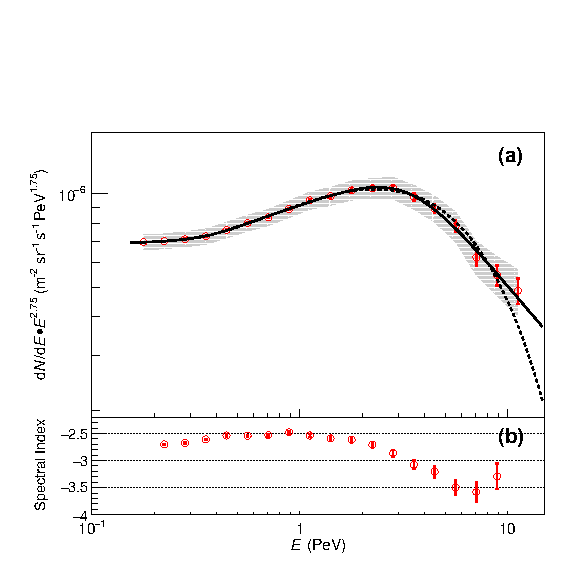
\includegraphics[width=0.66\hsize]{fig/lhaaso-proton-2025-fig2.pdf}
  \caption{LHAASO が測定した陽子エネルギースペクトル（上）と局所スペクトル指数（下）。赤点は測定値、灰色帯は系統的不確かさを表す。実線は二つの折れ曲がりをもつ一つの関数による適合で、三つの漸近的なべき乗区間を表す。破線は低い側の折れ曲がりと高い側の指数関数的カットオフを組み合わせた適合である。LHAASO Collaboration (2025) の Fig.~2 より引用~\cite{LHAASOProton2025}。}
  \label{fig:lhaaso_proton_spectrum}
\end{figure}

LHAASO は、同じエネルギー尺度で求めた陽子・ヘリウムの合計フラックスから陽子を差し引き、\(0.16\)--\(13\ \mathrm{PeV}\) のヘリウムスペクトルも測定した~\cite{LHAASOHelium2026}。EPOS-LHC に基づく結果では、\(1.05\pm0.05_{\mathrm{stat}}{}^{+0.22}_{-0.13}{}_{\mathrm{sys}}\ \mathrm{PeV}\) 付近に硬化、\(7.6\pm0.7_{\mathrm{stat}}\pm0.3_{\mathrm{sys}}\ \mathrm{PeV}\) 付近に軟化がある。フィットでは平滑化幅を固定し、位置を自由に求めている。陽子の選別と混入補正も更新しており、両核種の結果は統計的・系統的に独立ではない。また、別の相互作用モデルでは軟化位置が約 \(6.3\)--\(6.4\ \mathrm{PeV}\) となるため、EPOS-LHC で示した系統誤差だけを模型間の差全体と解釈することはできない。

\FloatBarrier

\subsection{Peters cycle と knee--second knee の接続}\label{subsec:peters_cycle}
全粒子スペクトルは異なる電荷をもつ成分の和である。
加速限界または銀河からの脱出がリジディティ \(\mathcal{R}\) で決まるなら、核種 \(Z\) の折れ曲がりエネルギーは
\begin{equation}
  E_{k,Z}\simeq Ze\mathcal{R}_c
  \label{eq:peters_scaling}
\end{equation}
と電荷に比例する。ここで \(\mathcal R_c\) は同じ源集団または伝搬過程に共通と仮定する特徴剛性である。
このため、陽子、ヘリウム、CNO 群、中間質量核、鉄群の各スペクトルが順次急峻化し、質量組成はエネルギーとともに重くなる。
各核種のスペクトルが電荷の順に折れ曲がるこの変化を Peters cycle と呼ぶ~\cite{Peters1961,Horandel2003}。

たとえば、核電荷 \(Z\) をもつ原子核のスペクトルを
\begin{equation}
  J_Z(E)
  =a_Z E^{-\gamma}
  \left[
    1+\left(\frac{E}{Ze\mathcal{R}_c}\right)^{\epsilon}
  \right]^{-\Delta\gamma/\epsilon}
  \label{eq:peters_component}
\end{equation}
と書けば、\(E\ll Ze\mathcal{R}_c\) では指数 \(\gamma\)、\(E\gg Ze\mathcal{R}_c\) では指数 \(\gamma+\Delta\gamma\) となる。
\(a_Z\) は核種ごとの規格化、\(\Delta\gamma>0\) は指数の増加量、\(\epsilon>0\) は折れ曲がりの鋭さを表す。
図~\ref{fig:peters_cycle}は、カットオフのエネルギーがリジディティに比例すると仮定した H\"orandel の poly-gonato モデルを示す。
この図では、直接観測から外挿した各質量群のスペクトルを合計し、全粒子スペクトルへ適合している。核電荷の小さい群から順に強度が急減し、knee から second knee に至る構造を作る~\cite{Horandel2003}。鉄より重い核種も含むため、鉄成分の軟化と、すべての銀河系内成分の終端は別の特徴となる。このモデルによる成分分解は、各核種のフラックスをそのエネルギーまで個別に測定した結果ではない。
同じ源集団と共通の特徴剛性を仮定し、LHAASO の陽子スペクトルに見られる \(3.3\ \mathrm{PeV}\) の急峻化を電荷に比例して延長すると、鉄に対応するエネルギーは約 \(8.6\times10^{16}\ \mathrm{eV}\) となる。これは条件付きの概算であり、全粒子スペクトルから鉄の最大剛性を測った結果ではない。この値は、KASCADE-Grande が報告した電子成分の少ない試料の折れ曲がりと数値的に整合する~\cite{KASCADEGrandeHeavyKnee2011,LHAASOProton2025}。
この対応は Peters cycle の \(Z\) 比例則と整合するが、すべての核種に共通する単一の基準リジディティを示したことにはならない。
ARGO-YBJ/LHAASO 試作機が測定した陽子・ヘリウム成分の折れ曲がりは約 \(0.7\ \mathrm{PeV}\) にあり、LHAASO の陽子スペクトル自体にも傾きの異なる複数の領域があるためである~\cite{ARGOYBJLHAASOLightKnee2015,LHAASOProton2025}。

\begin{figure}[htb]
  \centering
  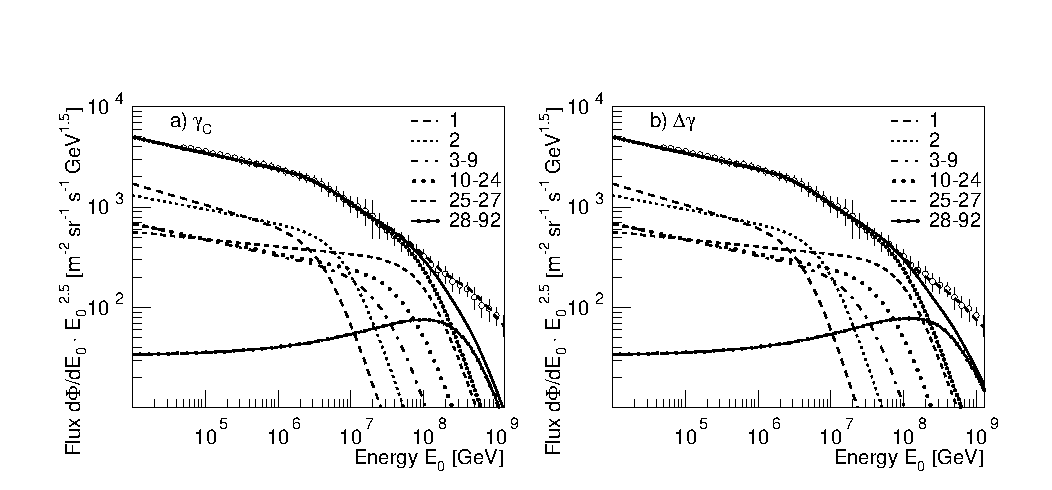
\includegraphics[width=0.92\hsize]{fig/horandel-2003-fig11.pdf}
  \caption{リジディティ依存のカットオフを仮定した poly-gonato モデルによる全粒子スペクトルと質量群別の寄与。左は全質量群でカットオフ後の指数 \(\gamma_c\) を共通とした場合、右は指数変化 \(\Delta\gamma\) を共通とした場合である。凡例の数字は核電荷 \(Z\) の範囲を表す。H\"orandel (2003) の Fig.~11 より引用~\cite{Horandel2003}。}
  \label{fig:peters_cycle}
\end{figure}

核電荷の順に折れ曲がる関係は、その原因が加速限界であっても、銀河磁場からの脱出であっても現れる。
前者では、式~\eqref{eq:hillas_condition}により最大エネルギーは \(Z\) に比例する。後者では、同じリジディティの粒子が同じ拡散係数をもつ。
どちらの機構からも似た全粒子スペクトルが生じるため、その形状だけでは加速限界と銀河磁場からの脱出を識別できない。
核種別スペクトル、\(\langle\ln A\rangle\)、異方性、および近傍 PeVatron が加速できる最高エネルギーを組み合わせれば、折れ曲がりのエネルギーが複数の電荷群で \(Z\) に比例するかを検証できる。
具体的に、Giacinti らの逃走モデルは、銀河磁場の規則成分と乱流成分を仮定して粒子軌道と逃走時間を求め、knee 以後の核種別スペクトルを説明する~\cite{Giacinti2015Escape}。この場合、核種ごとの軟化は逃走時間のリジディティ依存が変わることから生じ、源の最大リジディティを直接示すわけではない。
Mollerach と Roulet は、銀河系内の複数核種と低エネルギー側で抑制された銀河系外成分を重ね、knee から second knee の全粒子スペクトルと組成を記述した~\cite{Mollerach2019Knee}。このモデルでは、鉄成分の軟化、軽い核の寄与の減少、銀河系外成分の増加は、合計スペクトルと組成に異なる特徴を作る。核種の軟化位置、全粒子の硬化位置、組成の変化点を同じエネルギーとみなす必要はない。
相互作用断面積や粒子生成の変化も空気シャワーの再構成量に影響する。しかし、異なる検出手法で類似の構造が観測されているため、単一の検出器効果だけでは knee 系列を説明できない~\cite{PDGCosmicRays}。
\FloatBarrier

\subsection{Second knee 領域の観測}\label{subsec:second_knee_observations}
宇宙線強度が低い second knee 領域では、直接観測で十分な統計量を得られないため、空気シャワーからエネルギーと質量を推定する。質量の推定値はハドロン相互作用モデルに依存する。
Akeno と Fly's Eye は \((4\)--\(7)\times10^{17}\ \mathrm{eV}\) 付近の緩やかな急峻化を報告した~\cite{AkenoSpectrum1992,FlysEyeSpectrum1994,Horandel2003}。
\(8\times10^{16}\)--\(10^{17}\ \mathrm{eV}\) にも明瞭な構造が測定されており、second knee と呼ばれる特徴エネルギーは解析ごとに異なる。

KASCADE-Grande は観測面積を拡張し、\(10^{16}\)--\(10^{18}\ \mathrm{eV}\) の荷電粒子数とミューオン数を測定した~\cite{KASCADEGrandeDetector2010}。
2011 年の解析は、全荷電粒子数 \(N_{\mathrm{ch}}\) とミューオン数 \(N_\mu\) から質量に感度をもつ指標 \(k\) を構成し、天頂角 \(40^\circ\) 未満の事象を分類した。C と Si の MC 期待値の中間を境界とした重い核に富む試料では、\(\log_{10}(E/\mathrm{eV})=16.92\pm0.04\) に軟化が認められた。同じデータの全粒子スペクトルにも \(16.92\pm0.10\) の軟化があるが、論文による単一べき乗からのずれの有意性は、重い試料で \(3.5\sigma\)、全粒子で \(2.1\sigma\) と異なる~\cite{KASCADEGrandeHeavyKnee2011}。二つを独立した実験結果として数えることはできない。
2013 年の解析では、軽い核を強調するため、選別境界を He と CNO の間に変更した。その試料では \(\log_{10}(E/\mathrm{eV})=17.08\pm0.08\) に硬化が報告された~\cite{KASCADEGrandeLightAnkle2013}。論文は硬化がない場合の予測と観測事象数を Poisson 確率で比較し、\(5.8\sigma\) と評価している。この硬化は、全粒子スペクトルの second knee とは別の特徴である。
図~\ref{fig:kascade_grande_components}は、近接したエネルギー領域で、重い原子核に対応する試料が急峻化し、軽い原子核に対応する試料では傾きが緩やかになることを示す。

\begin{figure}[htb]
  \centering
  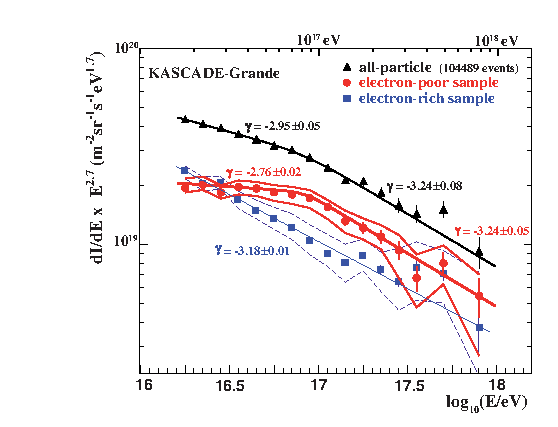
\includegraphics[width=0.49\hsize]{fig/kascade-grande-heavy-2011-fig4.pdf}\hfill
  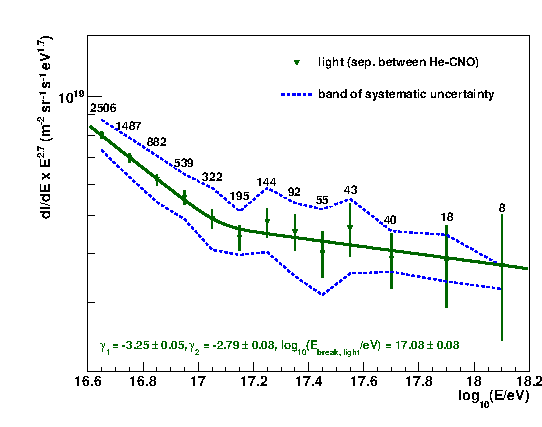
\includegraphics[width=0.49\hsize]{fig/kascade-grande-light-2013-fig5.pdf}
  \caption{KASCADE-Grande が再構成した質量群別エネルギースペクトル。左は全粒子、電子成分の少ない試料、電子成分の多い試料の比較であり、電子成分の少ない試料は約 \(8\times10^{16}\ \mathrm{eV}\) で急峻化する。右では、電子成分の多い試料のスペクトルの傾きが約 \(10^{17.08}\ \mathrm{eV}\) から緩やかになる。左図の帯は試料の選別条件による系統的不確かさを表し、エネルギー尺度の不確かさ全体を表すものではない。左は KASCADE-Grande Collaboration (2011) の Fig.~4、右は同 Collaboration (2013) の Fig.~5 より引用~\cite{KASCADEGrandeHeavyKnee2011,KASCADEGrandeLightAnkle2013}。}
  \label{fig:kascade_grande_components}
\end{figure}

TALE は、低エネルギー側では大気チェレンコフ光、高エネルギー側では大気蛍光を利用し、約 \(2\ \mathrm{PeV}\) から \(2\ \mathrm{EeV}\) までを同じ望遠鏡系で測定した。
位置を自由に求めたフィットでは、\(\log_{10}(E/\mathrm{eV})=16.22\pm0.017\) で硬化し、\(17.04\pm0.035\) で再び軟化する。後者の前後で指数は \(2.92\pm0.008\) から \(3.19\pm0.017\) へ変化し、second knee に対応する~\cite{TALESpectrum2018}。
図~\ref{fig:tale_second_knee}では、同一解析のエネルギースケール上で 2 つの折れ曲がりが示されている。

\begin{figure}[!htbp]
  \centering
  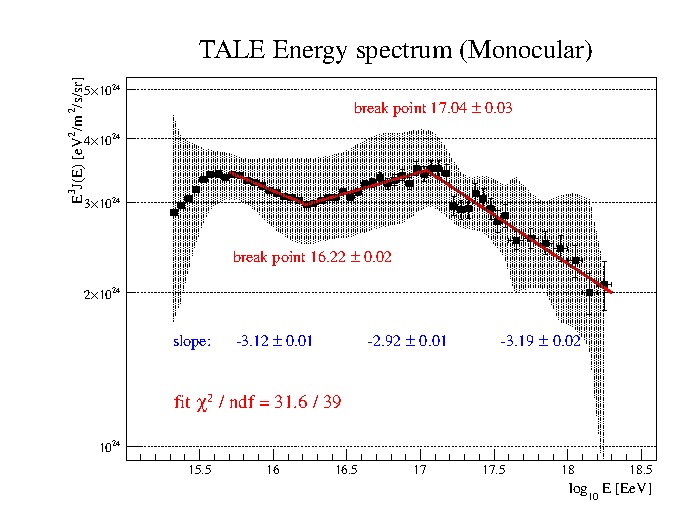
\includegraphics[width=0.64\hsize]{fig/tale-spectrum-2018-fig20.pdf}
  \caption{TALE 単眼解析による \(2\ \mathrm{PeV}\) から \(2\ \mathrm{EeV}\) の全粒子エネルギースペクトル。赤線は折れ曲がりを含む適合、灰色帯は系統的不確かさを表す。TALE Collaboration (2018) の Fig.~20 より引用~\cite{TALESpectrum2018}。}
  \label{fig:tale_second_knee}
\end{figure}

IceTop-73 の 2013 年解析は、地表信号から求めた全粒子スペクトルに \(130\pm30\ \mathrm{PeV}\) の軟化を報告した~\cite{IceTopSpectrum2013}。この位置は、別々のエネルギー区間にフィットしたべき乗の交点から求めている。地表と氷中の情報を組み合わせた 2019 年解析は組成も扱うが、観測期間が 2013 年解析と重なるため、独立した位置測定として重複計上しない~\cite{IceTopComposition2019}。
Tunka-133 は約 \(3\times10^{17}\ \mathrm{eV}\) で指数が \(2.99\pm0.01\) から \(3.29\pm0.09\) へ変わる形状を報告した~\cite{TunkaSpectrum2020}。高い側の位置について誤差を伴う推定値は示されていないため、ここでは概数による形状の報告として扱う。

Auger の \(433\ \mathrm{m}\) 間隔の地表アレイ（SD433）は、位置を自由、平滑化幅を固定したフィットにより、\(230\pm50_{\mathrm{stat}}\pm35_{\mathrm{sys}}\ \mathrm{PeV}\) の軟化を報告した~\cite{AugerSD4332023}。図~\ref{fig:auger433_spectrum}にそのスペクトルを示す。一方、\(750\ \mathrm{m}\) アレイの 2021 年解析は折れ曲がり位置を固定して高い側のスペクトル形状を評価しているため、独立に求めた位置の比較には加えない~\cite{AugerSecondKnee2021}。SD433 の尺度は SD750 を介して蛍光観測へ接続されており、両者の尺度も独立ではない。

\begin{figure}[!htbp]
  \centering
  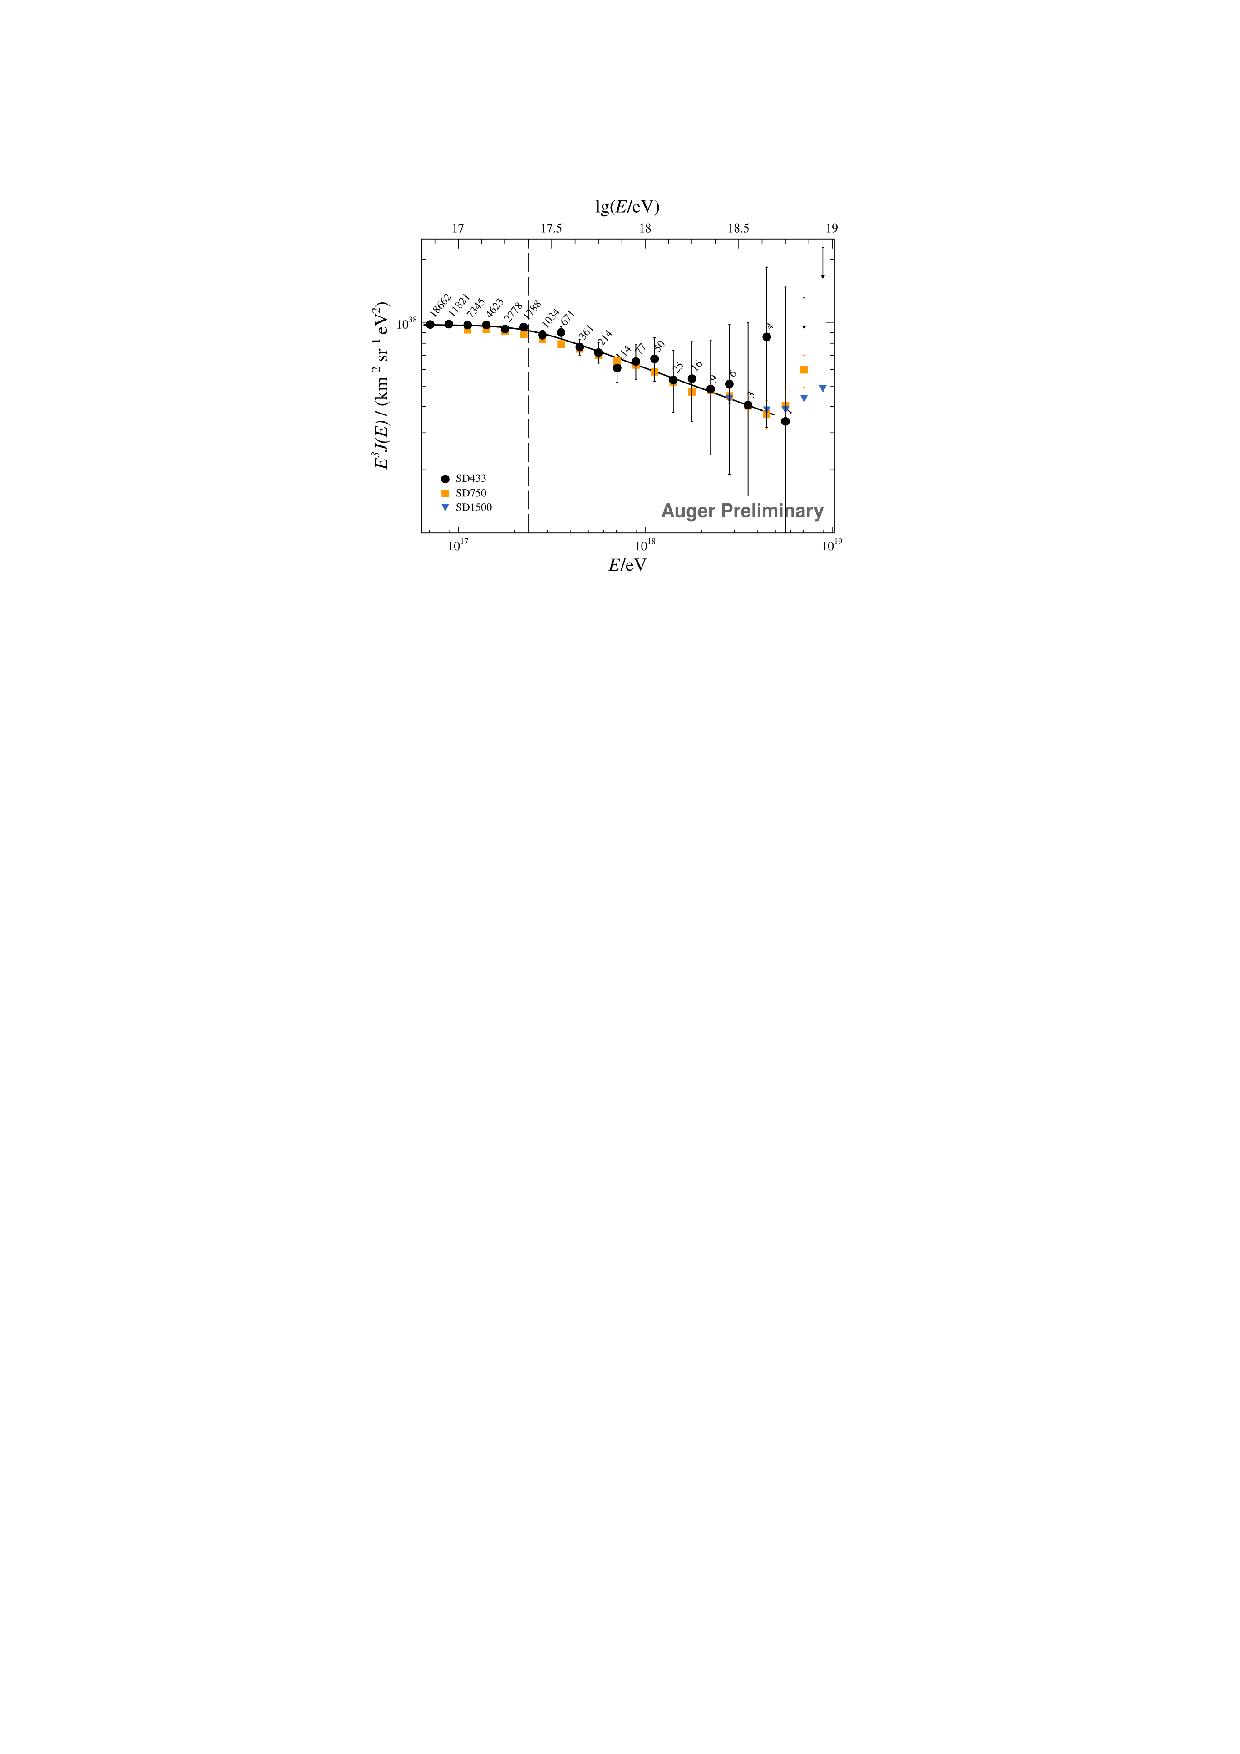
\includegraphics[width=0.62\hsize]{fig/auger-sd433-2023-fig5.pdf}
  \caption{Auger SD433 の全粒子スペクトル（黒点）とフィット（黒線）。橙点は SD750、青点は SD1500 の結果を示す。SD433 の誤差棒と上限は Feldman--Cousins 法による 90\% 信頼区間であり、縦破線は自由に求めた折れ曲がり位置を示す。G. Brichetto Orquera for the Pierre Auger Collaboration, PoS(ICRC2023)398, Fig.~5 より転載~\cite{AugerSD4332023}。\href{https://creativecommons.org/licenses/by-nc-nd/4.0/}{CC BY-NC-ND 4.0}。図の内容は変更していない。}
  \label{fig:auger433_spectrum}
\end{figure}

表~\ref{tab:second_knee_results}は全粒子スペクトルの位置推定を比較し、表~\ref{tab:composition_features}は異なる観測量の特徴を分けて示す。エネルギー尺度、分解能、選別、フィット関数が異なるため、全ての位置が同一の物理量を同じ精度で測っているわけではない。
\begin{table}[!htbp]
  \centering
  \small
  \caption{全粒子スペクトルの軟化位置の比較。\(x_b=\log_{10}(E_b/\mathrm{eV})\) とし、指数は \(J\propto E^{-\gamma}\) で定義する。TALE と KASCADE-Grande は論文のフィット誤差を示す。IceTop と Auger の指数は統計・系統誤差の順に記す。エネルギー尺度の系統誤差を全ての位置誤差へ加えた表ではない。}
  \label{tab:second_knee_results}
  \renewcommand{\arraystretch}{1.45}
  \begin{tabular}{@{}p{0.17\hsize}p{0.25\hsize}p{0.29\hsize}p{0.19\hsize}@{}}
    \hline
    実験・解析 & 軟化位置 & 前後の指数 \(\gamma\) & 推定方法 \\
    \hline
    \raggedright TALE 2018~\cite{TALESpectrum2018} & \raggedright \(x_b=17.04\pm0.035\) & \begin{tabular}[t]{@{}l@{}}\(2.92\pm0.008\) \\ \(\to3.19\pm0.017\)\end{tabular} & \raggedright 位置を自由にフィット \tabularnewline
    \raggedright KASCADE-Grande 2011~\cite{KASCADEGrandeHeavyKnee2011} & \raggedright \(x_b=16.92\pm0.10\) & \begin{tabular}[t]{@{}l@{}}\(2.95\pm0.05\) \\ \(\to3.24\pm0.08\)\end{tabular} & \raggedright 滑らかな折れ曲がりをフィット \tabularnewline
    \raggedright IceTop-73 2013~\cite{IceTopSpectrum2013} & \begin{tabular}[t]{@{}l@{}}\(E_b=(130\pm30)\) \\ \(\mathrm{PeV}\)\end{tabular} & \begin{tabular}[t]{@{}l@{}}\(2.903\pm0.010\pm0.03\) \\ \(\to3.374\pm0.069\pm0.08\)\end{tabular} & \raggedright 区間別べき乗の交点 \tabularnewline
    \raggedright Auger SD433 2023~\cite{AugerSD4332023} & \begin{tabular}[t]{@{}l@{}}\(E_b=230\ \mathrm{PeV}\) \\ \(\pm50_{\mathrm{stat}}\pm35_{\mathrm{sys}}\ \mathrm{PeV}\)\end{tabular} & \begin{tabular}[t]{@{}l@{}}\(3.00\pm0.05\pm0.10\) \\ \(\to3.32\pm0.08\pm0.10\)\end{tabular} & \raggedright 位置は自由、平滑化幅は固定 \tabularnewline
    \hline
  \end{tabular}
\end{table}

TALE の値は arXiv:1803.01288v1 の Table~5 に従い、同表のフィット誤差を示した。代表的なエネルギー尺度の不確かさ約 14--15\% は別の系統要因である。IceTop の位置誤差 \(30\ \mathrm{PeV}\) は、論文中で統計・系統に分解されていない。Akeno、Fly's Eye、Tunka の概数による報告と、位置を固定した Auger SD750 の解析も、測定方法を区別して比較する必要がある。

\begin{table}[!htbp]
  \centering
  \small
  \caption{全粒子の軟化とは区別する組成に関係した特徴。\(x_b=\log_{10}(E_b/\mathrm{eV})\) とする。KASCADE-Grande の誤差はフィット誤差であり、TALE の位置誤差は統計・系統の順に示す。}
  \label{tab:composition_features}
  \renewcommand{\arraystretch}{1.45}
  \begin{tabular}{@{}p{0.27\hsize}p{0.26\hsize}p{0.39\hsize}@{}}
    \hline
    実験・観測量 & 特徴の位置 & 変化と解釈上の条件 \\
    \hline
    \raggedright KASCADE-Grande 2011：重い核に富む試料~\cite{KASCADEGrandeHeavyKnee2011} & \raggedright \(x_b=16.92\pm0.04\) & \raggedright 指数 \(2.76\pm0.02\) から \(3.24\pm0.05\) への軟化。全粒子試料とデータを共有する \tabularnewline
    \raggedright KASCADE-Grande 2013：軽い核に富む試料~\cite{KASCADEGrandeLightAnkle2013} & \raggedright \(x_b=17.08\pm0.08\) & \raggedright 指数 \(3.25\pm0.05\) から \(2.79\pm0.08\) への硬化。2011 年とは選別境界も異なる \tabularnewline
    \raggedright TALE Hybrid 2026：\(\langle X_{\max}\rangle\)~\cite{TALEMassComposition2026} & \raggedright \(x_b=17.13\pm0.04\) \({}^{+0.05}_{-0.03}\) & \raggedright エロンゲーションレートの増加。全粒子スペクトルの位置測定ではなく、組成への換算は模型に依存する \tabularnewline
    \hline
  \end{tabular}
\end{table}
\FloatBarrier

\section{銀河系内成分から銀河系外成分への移行と超高エネルギー宇宙線}
\subsection{銀河系内成分から銀河系外成分への移行のモデル}\label{subsec:galactic_transition}
Second knee から ankle までの遷移を説明するモデルは複数あり、銀河系内成分が急減するエネルギーと、銀河系外成分が優勢になるエネルギーについて異なる予測を与える。
Ankle は Volcano Ranch 実験の John Linsley が 1963 年に初めて報告した。Linsley は同じ論文で、スペクトルの傾きが緩やかになるこの変化を、銀河系内成分と銀河系外成分の交差として解釈している~\cite{LinsleyAnkle1963,DelignyAnkle2014}。
現在、Auger と TA は ankle の位置と形状を大きな露出量で測定している。一方、その原因が銀河系内外成分の交差、対生成 dip、または源から放出される複数成分の重なりのいずれであるかは確定していない~\cite{AugerSpectrum2020,AugerTAEnergyScale2019}。
観測される全粒子強度を
\begin{equation}
  J(E)=J_{\mathrm{G}}(E)+J_{\mathrm{XG}}(E)
\end{equation}
として銀河系内成分と銀河系外成分の和で表すと、折れ曲がりは各成分固有の構造だけでなく、両成分の交差によっても生じる。銀河系外成分の出現、\(J_{\mathrm G}=J_{\mathrm{XG}}\) となる等寄与、銀河系内成分が無視できるほど小さくなる移行完了は、一般に異なるエネルギーを指す。全粒子スペクトルの second knee だけでは、これらの段階を一意に指定できない。

\paragraph{銀河系内成分が ankle まで延びるモデル}
このモデルは、標準的な超新星残骸成分より高い最大リジディティをもつ第 2 の銀河成分、いわゆる component B を導入する。銀河系外成分への主な遷移は ankle 付近に置かれる~\cite{Hillas2005}。
この第 2 成分は、EeV 近くまで宇宙線を加速できる銀河系内天体と、陽子から重い原子核までを含む組成を前提とする。
高リジディティ粒子は銀河磁場で強く閉じ込められないため、銀河面方向に予測される異方性の振幅がこのモデルを制約する。

追加銀河成分の組成も自明ではない。Thoudam らは、通常の超新星残骸成分に加え、銀河風の終端衝撃波での再加速や Wolf--Rayet 星の超新星を検討し、全粒子スペクトルと組成を比較した~\cite{Thoudam2016SecondGalactic}。後者では、second knee 付近から上で He や CNO が重要となり、鉄の寄与は小さくなり得る。したがって、追加銀河成分を導入することと、その源や組成を特定することは別の課題である。

\paragraph{Pair-production dip モデル}
銀河系外陽子は、宇宙マイクロ波背景放射との対生成反応
\begin{equation}
  p+\gamma_{\mathrm{CMB}}\rightarrow p+e^++e^-
\end{equation}
でエネルギーを失う。この過程によって EeV 領域のスペクトルに dip が形成され、その高エネルギー側が ankle として見える~\cite{BerezinskyDip2006}。
この場合、銀河系外陽子は ankle より低いエネルギーから寄与し、銀河系内成分から銀河系外成分への移行は second knee と ankle の間で進む。
明瞭な dip の形成には、銀河系外成分における陽子の優勢が必要である。質量組成の測定は、この条件を直接検証する。

\paragraph{混合組成・低最大リジディティモデル}
陽子から重核までを加速する銀河系外源を考える。最大エネルギーが \(E_{\max,Z}=Ze\mathcal{R}_{\max}\) に従うモデルでは、源からの脱出と伝搬中の光核分解によって組成は変化する。
Pierre Auger Observatory の \(5\ \mathrm{EeV}\) 以上のスペクトルと \(X_{\max}\) 分布を一様な源分布で同時適合すると、スペクトル指数の小さい注入スペクトルと比較的低い最大リジディティをもつ解が得られる。ただし、定量的結論は光核反応断面積、源分布、ハドロン相互作用モデルに依存する~\cite{AugerCombinedFit2017}。
この種のモデルでは、源から放出された二次陽子と一次の重い原子核が同じエネルギー領域へ寄与することによっても、ankle の形状が生じる。

源の周囲での光分解も、ankle 以下の軽成分を作る。Unger らは、加速された原子核が源周囲の光子場で相互作用し、低いエネルギーへ二次核子を供給するモデルを示した~\cite{Unger2015SourceEnvironment}。相互作用と逃走の時間尺度の競合により、ankle 以下の陽子とそれ以上の原子核が同じ源から生じ得るため、軽成分の増加を直ちに独立した一次陽子源の出現と同定することはできない。

\paragraph{Ankle 以下の成分と銀河系外磁場の効果}
Auger は \(6\times10^{17}\ \mathrm{eV}\) 以上のスペクトルと \(X_{\max}\) 分布を用い、ankle の上下を複数成分で記述した~\cite{Auger2023AcrossAnkle}。低い側の中間質量成分を銀河系内起源とするか銀河系外起源とするかには縮退が残り、スペクトルと組成だけでは一意に決まらない。この解析の下端は second knee の低い側を含まないため、second knee 全域を直接フィットした結果とも区別される。
銀河系外成分の低エネルギー側は、注入条件だけでなく、源間距離と伝播時間によっても変わる。低リジディティ粒子が磁場中を有限時間で十分に遠くまで伝播できない場合、地球へ到達するフラックスは抑制される。この magnetic-horizon 効果を含めると、スペクトルと組成から推定する源の注入条件が変化し得る~\cite{Auger2024MagneticHorizon}。ただし、結果は磁場と源集団の仮定に依存し、second knee の位置だけから銀河系外磁場を測定したことにはならない。

以上のモデルは排他的とは限らない。
現実には、複数種の銀河系内源と銀河系外源が同じエネルギー領域へ寄与する場合がある。この場合、second knee、軽い原子核のスペクトルに見られる ankle、全粒子 ankle は異なる遷移段階を表す可能性がある。
全粒子スペクトルに加えて、質量群別スペクトル、\(X_{\max}\) 分布、ミューオン数、銀河座標に対する異方性を同時に再現できるかどうかが、モデルを識別する鍵となる~\cite{PDGCosmicRays,Cristofari2023}。

\subsection{組成と異方性による移行の制約}\label{subsec:transition_anisotropy}
到来方向の異方性は、スペクトルと質量組成に加えて宇宙線の起源を制約する。Auger は 2020 年、約 \(0.03\ \mathrm{EeV}\) から \(32\ \mathrm{EeV}\) 以上までの赤経分布を調べ、双極子の赤道面内成分の振幅と位相を報告した~\cite{AugerAnisotropy2020}。これは \(8\ \mathrm{EeV}\) 以上の双極子検出より低いエネルギーにも測定範囲を広げ、移行領域を調べる情報を与える。
各起源成分の強度を \(J_i(E)\)、双極子ベクトルを \(\boldsymbol d_i(E)\) とすると、強度の和から得られる双極子は
\begin{equation}
  \boldsymbol d(E)=\frac{\sum_i J_i(E)\boldsymbol d_i(E)}{\sum_i J_i(E)}
  \label{eq:dipole_mixture}
\end{equation}
と表される。赤道面への投影についても同じ関係が成り立つ。したがって、観測される位相は各成分の強度だけでなく、双極子の大きさと方向にも依存する。異なる成分が部分的に打ち消し合う場合もあり、位相の変化を成分の等寄与点と同一視することはできない。
有意な振幅が検出されていない領域では、位相の推定値を確定した起源方向として扱うこともできない。Auger の同解析では、等方分布からその振幅以上が生じる確率が \(1\%\) より大きいエネルギー区間に、\(99\%\) 信頼水準の振幅上限を示している~\cite{AugerAnisotropy2020}。起源モデルは、この上限と組成の測定を、源の分布や磁場による偏向を含む予測に対して比較する必要がある。

Giacinti らは、銀河円盤内の源と複数の銀河磁場モデルについて粒子伝播を計算し、EeV 付近で銀河起源陽子が全フラックスを支配すると、予測される大規模異方性が観測上限を超えやすいことを示した~\cite{Giacinti2012Transition}。この制約は源分布と磁場の規則・乱流成分に依存し、重い原子核を含む全ての銀河成分の排除を意味しない。
Bister らは 2026 年のプレプリントの要旨で、ankle 以下の中間質量の原子核について、検討した定常・過渡的な銀河源モデルでは異方性が過大となり、銀河系外起源なら観測と整合すると報告している~\cite{Bister2026Transition}。また、second knee 付近の重い銀河成分の減少が双極子方向の変化に関係する可能性を論じている。これは検討した源と磁場のモデルに対する制約であり、全ての追加銀河成分が排除されたという一般的な結論ではない。

\subsection{超高エネルギー宇宙線の伝搬と観測}\label{subsec:uhecr_propagation}
銀河系外を伝搬する超高エネルギー宇宙線は、宇宙膨張による断熱損失に加え、背景光子との相互作用でエネルギーと核種を変える。
陽子では電子陽電子対生成に加え、十分高いエネルギーで
\begin{equation}
  p+\gamma_{\mathrm{CMB}}\longrightarrow \Delta^+\longrightarrow
  \begin{cases}
    p+\pi^0,\\
    n+\pi^+
  \end{cases}
\end{equation}
という光パイオン生成が起こる。
Greisen、Zatsepin、Kuzmin は 1966 年、宇宙マイクロ波背景放射との相互作用によって、数十 \(\mathrm{EeV}\) 以上の陽子が遠方から地球へ到達しにくくなることを指摘した~\cite{Greisen1966,ZatsepinKuzmin1966}。
原子核は、宇宙赤外・可視背景放射と宇宙マイクロ波背景放射による光核分解を受け、伝搬中に質量数 \(A\) が減少する~\cite{KoteraOlinto2011}。

予測から約 40 年後の 2008 年、HiRes は GZK カットオフを初めて \(5\sigma\) で観測したと報告した。同じ年、Auger も大統計の地表アレイを用いた独立の測定により、最高エネルギー側で宇宙線強度が急減することを確認した~\cite{HiResGZK2008,AugerSuppression2008}。
現在は Auger と TA がこの急減の形状を精密に測定している~\cite{AugerSpectrum2020,AugerTAEnergyScale2019,PDGCosmicRays}。
しかし、エネルギースペクトルの急減だけでは、伝搬中の GZK 効果と起源天体の最大リジディティを一意に分離できない。
GZK 効果は、宇宙線が伝搬できる距離と近傍宇宙の物質分布に応じて観測結果を変える。一方、最大リジディティが原因であれば、各核種のカットオフは \(Z\) に比例する。質量組成、到来方向、宇宙生成ニュートリノ、\(\gamma\) 線の上限は、両者を識別するための独立した情報を与える。

Auger は 2017 年、\(8\ \mathrm{EeV}\) 以上の大規模双極子異方性を \(5\sigma\) を超える有意度で観測した。双極子の方向は銀河中心と一致せず、このエネルギー領域で銀河系外起源が卓越することを支持する~\cite{AugerDipole2017}。
一方、個々の天体との対応は銀河・銀河間磁場による偏向と限られた統計量のため確立していない~\cite{AugerTA2023ArrivalDirections}。
Auger と TA のスペクトル比較では、各実験のエネルギースケールを系統誤差の範囲内で調整すると、共通視野における一致は改善する。一方、最高エネルギー側には残差がある~\cite{AugerTAEnergyScale2019}。
TA と Auger は主に北天と南天をそれぞれ観測しており、露出とエネルギースケールの違いが最高エネルギー領域の比較に残る~\cite{AugerTAEnergyScale2019}。

低エネルギーから knee 付近までは銀河系内起源が主要と考えられ、超新星残骸の衝撃波、星団風やスーパーバブル、パルサー関連天体などが候補に挙げられる~\cite{Gabici2019,PDGCosmicRays}。超新星残骸で得られる総エネルギーは銀河宇宙線を維持する供給量を満たすが、個々の残骸が陽子を PeV 領域まで加速できるかは未解決である。超高エネルギー \(\gamma\) 線観測は、銀河系内の PeVatron 候補を制約している~\cite{Cao2023}。

\paragraph{局所的な宇宙線と光子・ニュートリノによる制約}
地球で測定される荷電宇宙線のスペクトルが、銀河全体の平均と一致するとは限らない。Fang と Halzen は、近傍の限られた PeVatron の寄与によって、数 PeV の knee が局所的な特徴となる可能性を検討している~\cite{Fang2026LocalKnee}。この研究が直接扱うのは最初の knee であるが、地球で測った特徴を全ての銀河源に共通する最大リジディティへ直ちに置き換えないための例となる。
LHAASO の超高エネルギー光子観測は銀河系内の高エネルギー粒子集団を調べるが、光子の生成がハドロン相互作用によるのか、電子の放射によるのかを識別する必要がある~\cite{Cao2023}。IceCube が報告した銀河面方向のニュートリノ放射は、荷電宇宙線の局所スペクトルと異なる方法でハドロンの存在を制約する~\cite{IceCubeGalacticPlane2023}。ただし、銀河面信号が拡散放射と未分離の点源集団のどちらにどれだけ由来するかは、この検出だけでは決まらない。

Second knee から ankle 付近の \(0.1\)--\(10\ \mathrm{EeV}\) では、銀河系内成分の上限と銀河系外成分の増加が重なる。Ankle model、dip model、混合組成モデルは、この移行が起こるエネルギーと質量組成について異なる予測を与える~\cite{Cristofari2023,PDGCosmicRays}。TALE による \(10^{16.5}\)--\(10^{18.5}\ \mathrm{eV}\) の縦方向発達の測定は、この領域の組成を制約している~\cite{TALEMassComposition2026}。

数 EeV 以上では銀河系外起源が主要と考えられ、約 \(5\ \mathrm{EeV}\) より上の観測結果は重い原子核の寄与を示唆する。候補天体には活動銀河核、電波銀河、ガンマ線バースト、潮汐破壊現象、マグネター、銀河団降着衝撃波、スターバースト銀河などがある~\cite{GlobusBlandford2023}。\(8\ \mathrm{EeV}\) 以上の大規模双極子異方性も銀河系外起源を支持するが、個々の起源天体は同定されていない~\cite{AugerDipole2017,AugerTA2023ArrivalDirections}。

表~\ref{tab:source_by_energy}に、各エネルギー領域の代表的な起源候補と加速条件をまとめる。
\begin{table}[htb]
  \centering
  \small
  \caption{エネルギー領域ごとの代表的な宇宙線起源候補。いずれも確定した対応ではない。}
  \label{tab:source_by_energy}
  \begin{tabular}{@{}p{0.20\hsize}p{0.28\hsize}p{0.25\hsize}p{0.18\hsize}@{}}
    \hline
    エネルギー領域 & 主な起源候補 & 加速・伝搬上の条件 & 状況 \\
    \hline
    \(\mathrm{GeV}\)--\(\mathrm{TeV}\) & 銀河系内の超新星残骸、星形成領域、パルサー関連天体 & 衝撃波加速と銀河内拡散 & 伝搬の影響が大きく、個々の起源天体の同定は難しい \\
    \(\mathrm{TeV}\)--\(\mathrm{PeV}\) & 若い超新星残骸、銀河中心、星団風、スーパーバブル & PeVatron、リジディティに依存する最大エネルギー & 超高エネルギー \(\gamma\) 線観測が候補天体を制約 \\
    \(\mathrm{PeV}\)--\(\mathrm{EeV}\) & 銀河系内起源と銀河系外起源の宇宙線がともに寄与 & knee、second knee、遷移領域 & 組成測定が遷移の起こるエネルギーを制約 \\
    \(\gtrsim 5\ \mathrm{EeV}\) & 活動銀河核、電波銀河、GRB、TDE、マグネター、銀河団衝撃波、スターバースト銀河 & Hillas 条件、損失、脱出、磁場偏向 & 銀河系外起源が有力だが、個々の起源天体は未同定 \\
    \hline
  \end{tabular}
\end{table}

\FloatBarrier
\section{Second knee の未解決点と TALE-SD の研究目的}\label{sec:thesis_motivation}
全粒子スペクトルの軟化、質量群別スペクトルの変化、銀河系内起源の成分から銀河系外起源の成分への移行は、相互に関係し得るが、同じ観測事実ではない。軟化の位置だけから鉄成分の終端や起源成分の等寄与点を決めることはできず、その前後の指数と変化の幅を含むスペクトル形状を、組成と異方性の測定に対応づけることが課題となる。
TALE-SD による測定の目的は、地表粒子信号を用いて second knee をまたぐスペクトルを測り、TALE の光学観測によるスペクトルや縦方向発達と比較することである。同じ観測サイトで異なるシャワー成分を調べることは、共通するスペクトル構造と観測量・較正方法に依存する差を評価するうえで有用である~\cite{TALESpectrum2018,TALEMassComposition2026}。この比較には、検出効率、エネルギー分解能、組成とハドロン相互作用モデルに対する応答を含める必要がある。
次章では、各観測量と一次粒子のエネルギー・質量を結び付ける空気シャワー物理を導入し、地表信号からのエネルギー推定と較正方法を整理する。

\chapter{空気シャワーの物理と観測}\label{chap:air_shower}
PeV 以上では宇宙線強度が小さく、直接観測で十分な統計量を得ることが難しい。このため、空気シャワーの電磁成分、ミューオン成分、縦方向発達から一次粒子のエネルギーと質量を推定する。
本章では、電磁カスケードとハドロンカスケードの基本モデルを導入し、縦方向発達、横方向分布、シャワー前面と観測量との関係を述べる。
質量組成の推定では、ハドロン相互作用モデルへの依存とミューオン問題が主要な系統要因となる。

\section{空気シャワーとは何か}\label{sec:air_shower_overview}
エネルギーの高い宇宙線が地球大気に入射すると、大気中の原子核との相互作用によって多数の二次粒子が生成される。
生成された二次粒子はさらに相互作用や崩壊を繰り返し、大気中で増殖しながら広がる。
この粒子カスケードを空気シャワー（extensive air shower）という~\cite{PDGCosmicRays,Stanev2004}。
空気シャワーは一次粒子の運動量ベクトルを延長した軸（シャワー軸）に沿って発達し、その構造は次の 3 つの側面から記述される。
\begin{itemize}
  \item 大気中で粒子数がどのように増減するかを示す縦方向発達、
  \item 地表で粒子群がシャワー軸のまわりにどのように広がるかを示す横方向分布、
  \item シャワー軸から離れた粒子が軸付近の粒子よりどれだけ遅れて到来するかを示すシャワー前面
\end{itemize}

陽子や原子核の一次宇宙線が大気に入射すると、まず大気中の原子核とのハドロン相互作用を起こす~\cite{PDGCosmicRays,Matthews2005}。
この相互作用を起点としてパイオンや K 中間子などの二次粒子が多数生成され、シャワー全体が発達する。
したがって、空気シャワーは単一の粒子種からできているのではなく、ハドロン成分、電磁成分、ミューオン成分が相互に結び付いた複合系である~\cite{Matthews2005,Stanev2004}。

電磁シャワーは、主として電子・陽電子と光子からなるカスケードである。
高エネルギー光子は電子陽電子対生成を起こし、高エネルギー電子・陽電子は制動放射によって光子を放出する。
対生成と制動放射が繰り返されると、粒子数は増加し、各粒子のエネルギーは低下する~\cite{PDGPassage,Heitler1944}。
空気シャワー全体では、電子・陽電子と光子からなる電磁成分が粒子数で卓越しやすく、縦方向発達の極大と、シャワー軸に近い領域の横方向構造を強く支配する。
この電磁カスケードを特徴づける代表尺度が放射長 \(X_0\) である~\cite{PDGPassage,PDGAir}。

これに対してハドロンシャワーは、陽子や原子核のようなハドロンから始まる。
ハドロン相互作用では多数のパイオンが生成され、そのうち \(\pi^0\) は
\[
  \pi^0\to\gamma\gamma
\]
とただちに崩壊して電磁成分へエネルギーを移す。
一方、\(\pi^\pm\) や \(K^\pm\) はハドロン相互作用を継続するか、十分低エネルギーになると崩壊してミューオンとニュートリノを生む~\cite{Matthews2005,Montanus2013}。
このように、ハドロン相互作用で生成された二次粒子がエネルギーを運び、中性パイオンの崩壊が電磁カスケードを生む。荷電中間子の相互作用と崩壊の競合は、電磁成分へ移るエネルギーとミューオン・ニュートリノとして運ばれるエネルギーの割合を変える。

空気シャワーを記述するうえでは、電磁相互作用とハドロン相互作用で異なる長さ尺度が現れる。
電磁カスケードでは放射長 \(X_0\) を代表尺度とし、電子や光子の増殖・減衰が生じる深さスケールを表す。
これに対してハドロン成分では、相互作用長 \(\lambda_{\mathrm{int}}\) が次の相互作用までの深さを特徴づける~\cite{PDGPassage,PDGCosmicRays,Matthews2005}。
荷電パイオンや K 中間子における相互作用と崩壊の競合は、ミューオン数と時間構造を左右する~\cite{Matthews2005,Stanev2004}。

\section{空気シャワーの縦方向発達}\label{sec:longitudinal}
\subsection{Walter Heitler の電磁カスケードモデル}\label{subsec:heitler_em}
空気シャワーの縦方向発達は、大気深さ \(X\) の関数として記述する。
大気深さとは、シャワー軸に沿った距離 \(x\) に対して物質の密度 \(\rho(x)\) を積分した量である。基準点から距離 \(a\) までの大気深さは
\begin{equation}
  X(a) = \int_{0}^{a} \rho(x)\,\mathrm{d}x
\end{equation}
と表される。
大気深さを用いれば、大気密度の高度変化を取り込んでシャワー発達を記述できる。
このため、空気シャワーの発達は幾何学的距離ではなく、大気深さ（\(\mathrm{g\,cm^{-2}}\)）の関数として表す。

本稿で用いる \(X\)、\(X_0\)、\(X_{\max}\)、\(\lambda_{\mathrm{int}}\) などは、いずれも大気深さの次元をもつ。

\subsubsection{仮定}
電磁シャワーを記述する単純なモデルとして Heitler モデルを導入する。
Heitler モデルはハドロン相互作用やパイオン生成を含まず、電磁シャワーを次のように理想化する。
\begin{enumerate}
  \item 1 個の粒子は 1 世代後に 2 個の粒子になる。
  \item エネルギーは 2 個の粒子に等分される。
  \item 1 世代進むごとに、深さが一定量 \(d=X_0\ln 2\) だけ増える。
  \item 各粒子のエネルギーが臨界エネルギー \(E^\mathrm{crit}\) に達すると、それ以上の増殖は止まる。
\end{enumerate}

ここで \(X_0\) は放射長、\(d\) はモデルにおける分裂長、\(E^\mathrm{crit}\) は臨界エネルギー（critical energy）である。Heitler モデルでは、分裂長を \(d=X_0\ln 2\) と置く~\cite{Matthews2005,Montanus2013}。
放射長は、制動放射によって高エネルギー電子のエネルギーが平均で元の \(1/e\) になるまでの物質量として定義される。
Particle Data Group（PDG）の \textit{Atomic and Nuclear Properties of Materials} では、乾燥空気（1 気圧）に対する放射長は
\begin{equation}
  X_0 = 36.62\ \mathrm{g\,cm^{-2}}
\end{equation}
と与えられている~\cite{PDGAir}。
高エネルギー光子に対しては、放射長は電子陽電子対生成の長さ尺度としても用いられる。
PDG の \textit{Review of Particle Physics} によれば、光子の平均自由行程は近似的に \(9X_0/7\) である~\cite{PDGPassage}。
Heitler モデルでは、この放射長から定めた分裂長 \(d\) を用いて、電磁カスケードが深さとともに発達する速さを表す。

臨界エネルギーは、電子の制動放射によるエネルギー損失と電離損失とが同程度になる代表的なエネルギー尺度である。
電離損失の代表値を
\begin{equation}
  \left(\frac{\mathrm{d}E}{\mathrm{d}X}\right)_{\mathrm{ion}} \simeq 2\ \mathrm{MeV\,g^{-1}\,cm^2}
\end{equation}
とすると、臨界エネルギーは概ね
\begin{equation}
  E^\mathrm{crit} \sim X_0 \times 2\ \mathrm{MeV\,g^{-1}\,cm^2}
\end{equation}
で見積もれる。
空気では \(X_0 \simeq 36.7\ \mathrm{g\,cm^{-2}}\) であるから、
\begin{equation}
  E^\mathrm{crit} \sim 70\ \mathrm{MeV}
\end{equation}
となる。
PDG の表では、乾燥空気（1 気圧）に対する電子の臨界エネルギーは
\begin{equation}
  E^\mathrm{crit} = 81.76\ \mathrm{MeV}
\end{equation}
と与えられている~\cite{PDGAir}。
\subsubsection{粒子数、極大深さ、エロンゲーションレート}
一次粒子のエネルギーを \(E_0\) とすると、\(n\) 世代後の粒子数と一粒子あたりのエネルギーは
\begin{equation}
  N_n=2^n,\qquad \varepsilon_n=\frac{E_0}{2^n}
\end{equation}
である。増殖が止まる条件 \(\varepsilon_{n_{\max}}=E^{\mathrm{crit}}\) から、最大発達時の世代数と粒子数は
\begin{equation}
  n_{\max}=\frac{\ln(E_0/E^{\mathrm{crit}})}{\ln2},
  \qquad N_{\max}=\frac{E_0}{E^{\mathrm{crit}}}
\end{equation}
となる。分裂長 \(d=X_0\ln2\) を用いれば、極大深さは
\begin{equation}
  X_{\max}=n_{\max}d=X_0\ln\!\left(\frac{E_0}{E^{\mathrm{crit}}}\right)
  \label{eq:Xmax}
\end{equation}
と書ける。この純電磁モデルは、\(N_{\max}\propto E_0\) と \(X_{\max}\propto\ln E_0\) という基本的なスケーリングを与える~\cite{Heitler1944,Matthews2005}。ハドロン相互作用から始まる陽子シャワーの極大深さを、そのまま表す式ではない。

\(X_{\max}\) のエネルギー依存を表すエロンゲーションレートを
\begin{equation}
  D_{10}=\frac{\mathrm d X_{\max}}{\mathrm d\log_{10}(E_0/E_{\mathrm{ref}})}
\end{equation}
と定義する。\(E_{\mathrm{ref}}\) は対数の引数を無次元にする固定した基準エネルギーであり、微分の値はその選択によらない。\(D_{10}\) はエネルギーの常用対数が 1 増えるときの極大深さの変化を表し、大気深さの単位をもつ。式~\eqref{eq:Xmax}から、このモデルでは \(D_{10}=X_0\ln10\) となる。拡散係数 \(D\) とは異なる量である。

\subsection{Walter Heitler--James Matthews モデル}\label{subsec:heitler_matthews}

\subsubsection{ハドロン相互作用の導入}
前節では、1 世代進むごとに粒子数が 2 倍になり、各粒子のエネルギーが半分になると仮定した。
Heitler--Matthews モデルは、一次粒子と大気の衝突による多数のパイオン生成を電磁モデルに導入し、ハドロンシャワーの発達を記述する~\cite{Matthews2005,Montanus2013}。
最初のハドロン相互作用が起こる深さは、相互作用長 \(\lambda_{\mathrm{int}}\) によって特徴づけられる。相互作用深さを指数分布で表すと、深さ \(X\) まで相互作用せずに到達する一次粒子の確率は
\begin{equation}
  P(X_1>X)=\exp\!\left(-\frac{X}{\lambda_{\mathrm{int}}}\right)
\end{equation}
と書ける。ここで \(X_1\) は最初の相互作用深さであり、\(\lambda_{\mathrm{int}}\) はその平均値である。したがって、相互作用長は次の相互作用が起こる深さの尺度を与える。

放射長 \(X_0\) が電磁シャワーの発達尺度を与えるのに対し、相互作用長 \(\lambda_{\mathrm{int}}\) はハドロンシャワーの開始深さを特徴づける。
また、大気原子核との相互作用断面積は一次粒子の核種によって異なる。
原子核半径が概ね \(A^{1/3}\) に比例するとみなせば、幾何学的な見積もりでは断面積の質量数依存は \(A^{2/3}\) 程度になる。
そのため、重い原子核ほど原子核--空気相互作用断面積が大きく、平均自由行程は短くなりやすい。
これは、重い原子核によるシャワーが比較的浅い深さで始まりやすいことの一因である~\cite{Matthews2005,Stanev2004,PDGCosmicRays}。
ただし、実際の原子核--空気断面積は単純な幾何学だけで決まるわけではなく、Glauber 型の扱いや高エネルギーハドロン相互作用モデルに依存する。

最も単純には、1 回のハドロン相互作用で合計 \(N_{\mathrm{tot}}\) 個のパイオンが生じ、
そのうち
\[
  N_{\mathrm{ch}}=\frac{2}{3}N_{\mathrm{tot}},
  \qquad
  N_{\pi^0}=\frac{1}{3}N_{\mathrm{tot}}
\]
がそれぞれ荷電パイオンと中性パイオンであるとする~\cite{Matthews2005}。
中性パイオンはただちに
\[
  \pi^0\to \gamma\gamma
\]
と崩壊してエネルギーを電磁成分へ移し、荷電パイオンはハドロンカスケードを継続する。
Heitler--Matthews モデルでは、各世代のエネルギーが
\[
  E_{\mathrm{had}}\to \frac{2}{3}E_{\mathrm{had}},
  \qquad
  E_{\mathrm{em}}\to E_{\mathrm{em}}+\frac{1}{3}E_{\mathrm{had}}
\]
とハドロン成分と電磁成分に分配される。

このエネルギー分配から、電磁成分とハドロン成分の割合を大まかに見積もれる。
\(n\) 世代後のハドロン成分のエネルギーは
\begin{equation}
  E_{\mathrm{had}}(n)=\left(\frac{2}{3}\right)^n E_0
\end{equation}
であり、そこまでに電磁成分へ移った累積エネルギーは
\begin{equation}
  E_{\mathrm{em}}(n)=E_0-E_{\mathrm{had}}(n)=\left(1-\left(\frac{2}{3}\right)^n\right)E_0
\end{equation}
となる。
各成分のエネルギー割合は
\begin{equation}
  f_{\mathrm{had}}(n)=\left(\frac{2}{3}\right)^n,
  \qquad
  f_{\mathrm{em}}(n)=1-\left(\frac{2}{3}\right)^n
\end{equation}
と見積もれる~\cite{Matthews2005,Stanev2004}。

たとえば 1 世代後には
\[
  f_{\mathrm{em}}=\frac{1}{3},
  \qquad
  f_{\mathrm{had}}=\frac{2}{3}
\]
であり、2 世代後には
\[
  f_{\mathrm{em}}=1-\left(\frac{2}{3}\right)^2=\frac{5}{9}
\]
となる。
数世代後には、エネルギーの大部分が電磁成分へ移る。

ただし、ここでの見積もりはエネルギー割合を対象とし、ある深さに存在する粒子数の割合を表さない。
粒子数で見ると、\(\pi^0\to\gamma\gamma\) を起点とする電磁カスケードから大量の \(e^\pm\) と \(\gamma\) が生じ、電磁成分はハドロン成分を大きく上回る。

\subsubsection{重ね合わせモデルと質量組成}
重ね合わせモデルでは、全エネルギー \(E_0\) をもつ質量数 \(A\) の原子核を、エネルギー \(E_0/A\) の核子 \(A\) 個が同時に入射したものとして扱う。これにより、原子核シャワーの極大深さを、より低いエネルギーの陽子シャワーに対応づけて
\begin{equation}
  X_{\max}^{(A)}(E_0)\simeq X_{\max}^{(p)}(E_0/A)
\end{equation}
と近似する~\cite{Matthews2005,Montanus2013}。さらに陽子のエネルギー依存に純電磁モデルと同じ対数形を仮定すれば、質量による差は模式的に \(-X_0\ln A\) となる。しかし、実際の陽子シャワーはハドロン相互作用から始まるため、放射長 \(X_0\) を質量に対する応答係数として普遍的に用いることはできない。

相互作用モデルの質量への応答を区別するため、対象エネルギーで核種ごとの平均を \(\ln A\) の一次式で近似する場合を考える。この仮定の下では、
\begin{equation}
  \langle X_{\max}\rangle(E)
  \simeq\langle X_{\max}\rangle_p(E)
  -F(E)\langle\ln A\rangle(E)
  \label{eq:xmax_mass_response}
\end{equation}
と表す~\cite{AugerXmaxInterpretation2013}。同論文の係数 \(f_E\) に対して \(F=-f_E\) と定義した。\(\langle X_{\max}\rangle_p\) は陽子シャワーの予測平均、\(F(E)\) は大気深さの次元をもつ質量への応答係数であり、いずれもハドロン相互作用モデルに依存する。検出器の受容と再構成の影響も、比較する測定に合わせて扱う必要がある。係数を数値的に用いる場合は、そのモデルの評価範囲を確認し、低いエネルギーへ無条件に外挿しない。

\(x=\log_{10}(E/E_{\mathrm{ref}})\) とし、\(D_{10,p}=\mathrm d\langle X_{\max}\rangle_p/\mathrm dx\) を定義すると、
\begin{equation}
  D_{10}=D_{10,p}-\frac{\mathrm dF}{\mathrm dx}\langle\ln A\rangle
  -F\frac{\mathrm d\langle\ln A\rangle}{\mathrm dx}
\end{equation}
を得る。\(F>0\) なら、他の条件が同じとき、組成が軽くなる変化は最後の項を通じてエロンゲーションレートを増やす。ただし、陽子の予測と \(F\) 自体のエネルギー依存も関係するため、測定された傾きだけでは組成変化を一意に決められない。

純電磁モデルの最大粒子数を各核子へ形式的に適用すれば、重ね合わせによって \(N_{\max}^{(A)}\simeq A(E_0/A)/E^{\mathrm{crit}}=E_0/E^{\mathrm{crit}}\) となる。この単純化では最大粒子数の質量依存が消えるが、実際の最大電子数の規格化と粒子の定義は次項で区別する。

図~\ref{fig:xmax_pdg}に、複数の実験で測定された \(\langle X_{\max}\rangle\) とその揺らぎを示す。
軽い一次粒子は平均的に深い \(X_{\max}\) をもち、重い一次粒子は浅い \(X_{\max}\) をもつ。
また、陽子のような軽い一次粒子では最初の相互作用深さやシャワー発達の揺らぎが大きいため、\(X_{\max}\) 分布の幅も大きくなりやすい。
このため、\(\langle X_{\max}\rangle\) と \(\sigma(X_{\max})\) は、質量組成を推定するための基本的な観測量である~\cite{PDGCosmicRays,TALEMassComposition2026}。

\begin{figure}[htb]
  \centering
  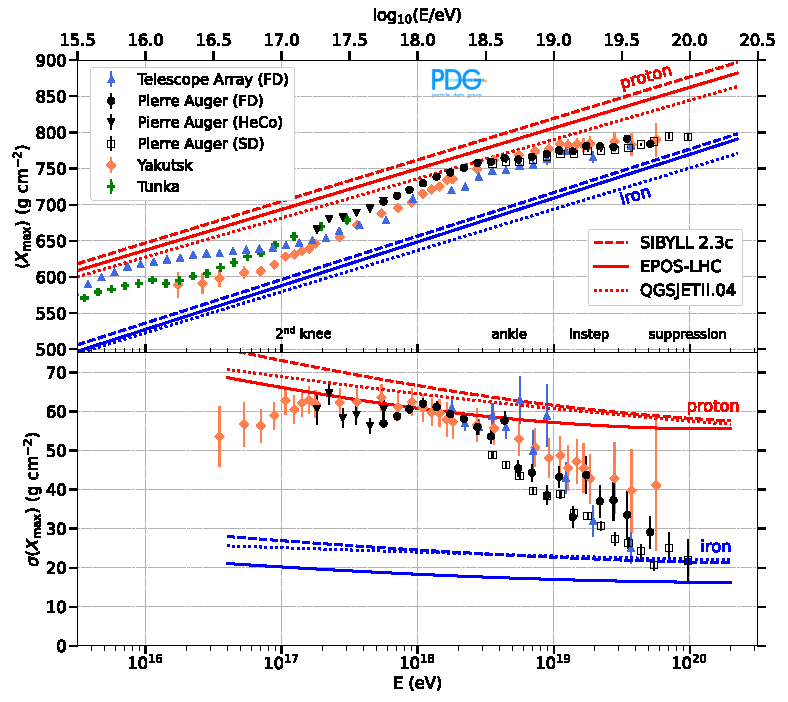
\includegraphics[width=0.85\hsize]{fig/Xmax.pdf}
  \caption{\(\langle X_{\max}\rangle\) と \(\sigma(X_{\max})\) のエネルギー依存。PDG のレビュー \textit{Cosmic Rays} の Fig.~30.8 より引用~\cite{PDGCosmicRays}。}
  \label{fig:xmax_pdg}
\end{figure}

\subsubsection{電子数とミューオン数}
Heitler モデルでは、電磁シャワーの最大粒子数 \(N_{\max}^{\mathrm{em}}\) は
\[
  N_{\max}^{\mathrm{em}}=\frac{E_0}{E^\mathrm{crit}}
\]
であり、空気中の臨界エネルギー \(E^\mathrm{crit}\simeq 0.08\,\mathrm{GeV}\) を代入すると
\[
  N_{\max}^{\mathrm{em}}\simeq 12.5\,\frac{E_0}{\mathrm{GeV}}
\]
となる。
ここでの \(N_{\max}^{\mathrm{em}}\) は、電子・陽電子と光子を区別しない Heitler モデルの粒子数である。実際の最大電子数 \(N_e^{\max}\) と比較するには、電子・陽電子を数えるエネルギーしきい値と、電子数が最大となる深さを定義する必要がある。
ハドロンシャワーでは、異なる深さで生成される電磁サブシャワーの重なりと、ハドロン・ミューオン成分へのエネルギー分配が電子数に影響する。\(N_e^{\max}\) が一次エネルギーにほぼ比例するという関係は有用だが、その比例係数は粒子の定義とモデル条件に依存する~\cite{Matthews2005,Montanus2013}。純電磁モデルとの係数の差を、エネルギー分配だけに帰属させることはできない。

Heitler--Matthews モデルでは、十分低エネルギーになった荷電パイオンがハドロン相互作用を継続せず、崩壊してミューオンを生成する。
荷電パイオンのエネルギーが臨界エネルギー \(E_\pi^{\mathrm{crit}}\) まで下がると、
各荷電パイオンは 1 個のミューオンを与えると仮定する~\cite{Matthews2005}。

1 世代で荷電パイオンの数は \(N_{\mathrm{ch}}\) 倍になり、
第 \(n\) 世代での各荷電パイオンのエネルギーは
\[
  E_n = \frac{E_0}{N_{\mathrm{tot}}^n}
\]
と近似できる。
崩壊が始まる世代数 \(n_c\) は
\begin{equation}
  \frac{E_0}{N_{\mathrm{tot}}^{n_c}}=E_\pi^{\mathrm{crit}}
\end{equation}
より
\begin{equation}
  n_c = \frac{\ln(E_0/E_\pi^{\mathrm{crit}})}{\ln N_{\mathrm{tot}}}
\end{equation}
である。

このときミューオン数は、その世代での荷電パイオン数に等しいとみなして
\begin{align}
  N_\mu
  &= N_{\mathrm{ch}}^{n_c} \\
  &= \exp\!\left(n_c\ln N_{\mathrm{ch}}\right) \\
  &= \exp\!\left(\ln\!\left(\frac{E_0}{E_\pi^{\mathrm{crit}}}\right)
     \frac{\ln N_{\mathrm{ch}}}{\ln N_{\mathrm{tot}}}\right) \\
  &= \left(\frac{E_0}{E_\pi^{\mathrm{crit}}}\right)^{\beta}
\end{align}
と書ける。
ただし
\begin{equation}
  \beta = \frac{\ln N_{\mathrm{ch}}}{\ln N_{\mathrm{tot}}}
\end{equation}
である。

Matthews の単純モデルと同様に \(N_{\mathrm{ch}}=10\)、\(N_{\mathrm{tot}}=15\) とすると
\[
  \beta = \frac{\ln 10}{\ln 15}\simeq 0.85
\]
が得られる~\cite{Matthews2005}。
この関係から、ミューオン数は
\begin{equation}
  N_\mu \propto E_0^{\beta},
  \qquad
  \beta\simeq 0.85
\end{equation}
となる。指数 \(\beta\) は 1 より小さいため、ミューオン数はエネルギーに比例する場合よりも緩やかに増加する。より現実的な多重度を用いた場合も、\(\beta\) は概ね \(0.85\)--\(0.95\) の範囲にある~\cite{PDGCosmicRays}。

質量数 \(A\) の一次粒子に対しては、直前に導入した重ね合わせモデルを用いる~\cite{Matthews2005,Montanus2013,Stanev2004}。
このときミューオン数は
\begin{align}
  N_\mu^{(A)}(E_0)
  &\simeq A\left(\frac{E_0/A}{E_\pi^{\mathrm{crit}}}\right)^{\beta} \\
  &= A^{1-\beta}\left(\frac{E_0}{E_\pi^{\mathrm{crit}}}\right)^{\beta}
\end{align}
となる~\cite{Matthews2005,Montanus2013}。
同じ全エネルギー \(E_0\) の空気シャワーでは、重い原子核ほどミューオン数が多くなる~\cite{Matthews2005,Montanus2013}。

\subsection{ミューオン問題とエネルギー・組成の推定}\label{subsec:muon_puzzle}
Heitler--Matthews モデルが示すように、地上ミューオン数は一次エネルギーと質量の双方に感度をもつ。
現実の解析では、LHC データを用いて調整したハドロン相互作用モデルを空気シャワーシミュレーションへ外挿する。
しかし、複数の実験では、\(X_{\max}\) などと整合する質量組成を仮定しても、モデル予測が観測されたミューオン量に届かない。
この系統的な不一致をミューオン問題、または muon deficit problem と呼ぶ~\cite{DembinskiMuon2019,AlbrechtMuonPuzzle2022}。
Auger は 2015 年、ハイブリッド観測から UHECR シャワーの平均ミューオン数を求めた。\(X_{\max}\) と整合する質量組成を仮定しても、観測値は現行モデルの予測を上回った~\cite{AugerMuon2015}。
8 実験による共通尺度のメタ解析は、この不一致が特定の実験だけに現れるのではなく、エネルギーとともに増大することを示した~\cite{DembinskiMuon2019}。

実験間の比較では、検出器応答を通したミューオン量 \(N_\mu^{\mathrm{det}}\) を、同じ条件の陽子と鉄の予測を用いて
\begin{equation}
  z=\frac{\ln N_\mu^{\mathrm{det}}-\ln N_{\mu,p}^{\mathrm{det}}}
  {\ln N_{\mu,\mathrm{Fe}}^{\mathrm{det}}-\ln N_{\mu,p}^{\mathrm{det}}}
  \label{eq:muon_z}
\end{equation}
と規格化する~\cite{DembinskiMuon2019}。データと両核種の予測で、用いるミューオン量、選別、平均の取り方を一致させる必要がある。特に \(\ln\langle N_\mu\rangle\) と \(\langle\ln N_\mu\rangle\) は一般に異なる。
重ね合わせモデルの \(N_\mu\propto A^{1-\beta}E^\beta\) は、固定エネルギーにおいて \(\langle\ln N_\mu\rangle\) が \(\langle\ln A\rangle\) の一次式となることを示す。この近似に基づく組成の基準値は
\begin{equation}
  z_{\mathrm{mass}}\simeq\frac{\langle\ln A\rangle}{\ln56}
\end{equation}
である。一方、平均してから対数を取る場合には、\(\kappa=1-\beta\) として \(\ln\langle A^\kappa\rangle/(\kappa\ln56)\) が現れ、組成分布の幅にも依存する。実際の比較にはシャワーの揺らぎ、エネルギービンの幅、検出器応答が関係するため、\(z_{\mathrm{mass}}\) を全ての実験の \(z\) と厳密に同じ量とみなすことはできない。
ミューオン問題とは、\(X_{\max}\) などで制約された質量組成から期待される値よりも、観測されたミューオン指標が系統的に大きいという不一致である。

このメタ解析によると、約 \(10\ \mathrm{PeV}\) より上では、データと LHC の測定結果に基づいて調整された相互作用モデルとの差がエネルギーとともに増大した。その傾きは EPOS-LHC と QGSJetII-04 の双方に対して有意であった~\cite{DembinskiMuon2019}。
図~\ref{fig:muon_meta_analysis}は、質量組成から期待される \(z_{\mathrm{mass}}\) を差し引いた \(\Delta z=z-z_{\mathrm{mass}}\) が、両モデルに対してエネルギーとともに増加することを示す。

\begin{figure}[htb]
  \centering
  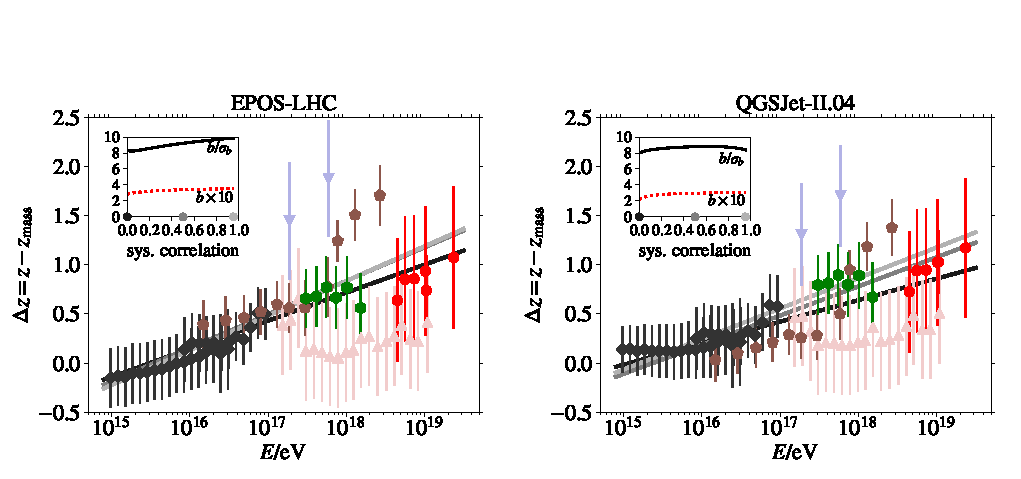
\includegraphics[width=0.92\hsize]{fig/dembinski-muon-2019-fig10.pdf}
  \caption{8 つの空気シャワー実験によるミューオン測定を共通尺度で比較したメタ解析。縦軸は質量組成の期待値を差し引いた \(\Delta z=z-z_{\mathrm{mass}}\)、横軸は一次エネルギーである。左は EPOS-LHC、右は QGSJetII-04 に対する比較を示す。直線は実験内の系統的不確かさの相関を変えた適合であり、KASCADE-Grande と EAS-MSU の点はエネルギースケールを相互較正していない。Dembinski et al. (2019) の Fig.~10 より引用~\cite{DembinskiMuon2019}。}
  \label{fig:muon_meta_analysis}
\end{figure}

Auger の \(6\)--\(16\ \mathrm{EeV}\) のハイブリッド事象では、縦方向発達をデータに合わせても、地表のハドロン由来信号を EPOS-LHC に対して \(1.33\pm0.16\) 倍、QGSJetII-04 に対して \(1.61\pm0.21\) 倍に増やす必要があった~\cite{AugerHadronic2016}。
レビューは、不一致が顕在化するシャワーエネルギーを約 \(40\ \mathrm{PeV}\) と整理している~\cite{AlbrechtMuonPuzzle2022}。陽子を一次粒子とし、静止核子との衝突に高エネルギー近似 \(\sqrt{s_{NN}}\simeq\sqrt{2m_pc^2E_0}\) を用いると、これは核子間重心系エネルギー約 \(8\)--\(9\ \mathrm{TeV}\) に対応する。ここで \(m_p\) は陽子質量である。質量数 \(A\) の原子核では、核子あたりのエネルギー \(E_0/A\) を用いる必要がある。不一致が顕在化する一次エネルギーを、個々のハドロン衝突における新しい反応の厳密なしきい値と同一視することはできない。
核子間重心系エネルギーが LHC の到達範囲にあっても、空気シャワーでは、加速器実験で十分に制約されていない超前方粒子生成が各世代で繰り返される。このため、衝突エネルギーだけではモデルの信頼性を保証できない。

各ハドロン相互作用から電磁成分へ移るエネルギー割合が減ると、ハドロンカスケードの残存エネルギーは増え、地上のミューオン数も増加する。
候補として、バリオン・反バリオンやストレンジ粒子の生成量、荷電粒子多重度、前方領域の \(\pi^0\) 生成率の修正などが議論されている~\cite{AlbrechtMuonPuzzle2022}。
Heitler--Matthews モデルの関係 \(N_\mu\propto N_{\mathrm{ch}}^{n_c}\) が示すように、1 回の相互作用における小さなエネルギー分配差でも、世代ごとに累積してミューオン数の大きな差となりうる。
ただし、ミューオン数だけを合わせる修正が \(X_{\max}\)、その揺らぎ、地上電磁信号、加速器データを同時に再現するとは限らない。

Second knee に近い領域では、Auger の地下ミューオン検出器（UMD）が \(2\times10^{17}\)--\(2\times10^{18}\ \mathrm{eV}\) のミューオン密度を直接測定した。基準角に換算した密度と \(\langle X_{\max}\rangle\) を組み合わせると、EPOS-LHC と QGSJetII-04 の予測は測定値を同時には再現しない~\cite{AugerUMD2020}。この測定が扱うのはミューオン密度であり、シンチレータの全信号や \(S_{600}\) の倍率ではない。
図~\ref{fig:auger_umd_xmax}は、基準角 \(35^\circ\) へ換算した軸距離 \(450\ \mathrm{m}\) のミューオン密度 \(\rho_{35}\) と平均 \(X_{\max}\) の比較である。ミューオン観測と蛍光観測の結果を同じエネルギーで比較しており、全て同一事象の同時測定を示す図ではない。
\begin{figure}[htb]
  \centering
  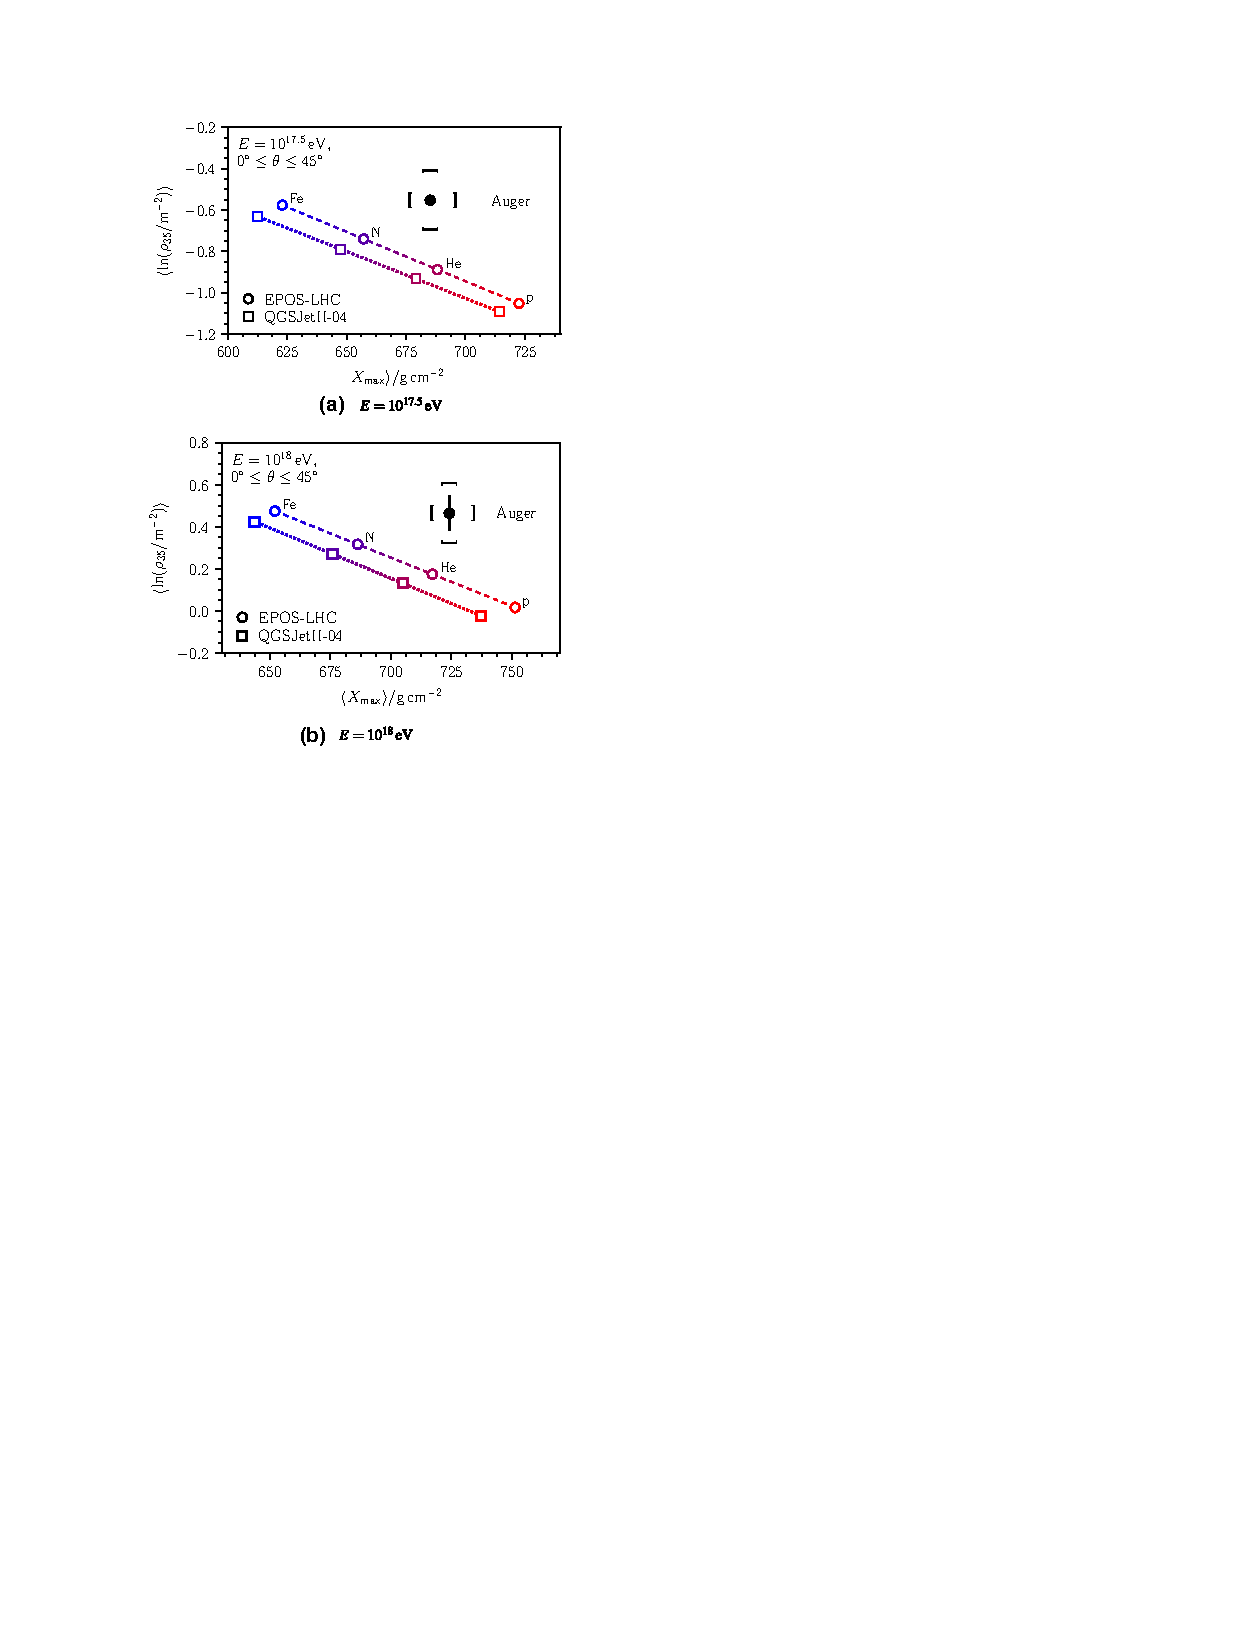
\includegraphics[width=0.49\hsize]{fig/auger-umd-2020-fig12.pdf}
  \caption{Auger UMD の \(\langle\ln(\rho_{35}/\mathrm{m^{-2}})\rangle\) と蛍光観測の \(\langle X_{\max}\rangle\) の比較。上は \(10^{17.5}\ \mathrm{eV}\)、下は \(10^{18}\ \mathrm{eV}\) に対応する。黒点と誤差棒は測定値と統計誤差、括弧は系統誤差を示す。色点は p、He、N、Fe の予測で、丸・破線は EPOS-LHC、四角・点線は QGSJetII-04 を表す。A. Aab et al., Eur. Phys. J. C 80, 751 (2020), Fig.~12 より転載~\cite{AugerUMD2020}。\href{https://creativecommons.org/licenses/by/4.0/}{CC BY 4.0}。図の内容は変更していない。}
  \label{fig:auger_umd_xmax}
\end{figure}

Bellido らは、SUGAR と Auger が同じ南天の宇宙線スペクトルを測ると仮定し、Auger のエネルギースケールを基準に、\(10^{17}\)--\(10^{18.5}\ \mathrm{eV}\) における SUGAR のミューオン数とエネルギーの関係を求めた。その比較では、MC に対するミューオン量のずれにエネルギー依存が認められた~\cite{BellidoSUGAR2018}。これはスペクトルの対応から換算関係を制約した結果であり、同一事象のミューオン数を両実験で比較したものではない。

この問題は second knee の解釈に影響する。
KASCADE-Grande のような解析は、荷電粒子数とミューオン数の相関を用いて試料を軽い原子核と重い原子核に対応する群へ分類する。シミュレーションがミューオン数を過小評価すれば、この相関に基づく質量の推定が重い側へ偏り得る。また、組成に依存する地表信号の補正を通じて、エネルギースケールも変化しうる。
このため、second knee 付近の質量群別スペクトルの解釈は、相互作用モデルだけでなく、\(X_{\max}\)、地表電磁成分、異なるしきい値で測定したミューオン成分との整合性にも依存する。地表信号のエネルギー換算への影響は、検出器中のミューオン信号の割合を通じて評価する必要があり、第\ref{sec:energy_calibration}節でその関係を述べる。

\subsection{縦方向発達の経験関数}\label{subsec:gh}

\subsubsection{関数形と各パラメータ}
空気シャワーの縦方向発達全体を表す経験式として、Thomas K. Gaisser と Anthony Michael Hillas による Gaisser--Hillas 関数~\cite{GaisserHillas1977}
\begin{equation}
  N(X)=N_{\max}
  \left(\frac{X-X_0^{\mathrm{GH}}}{X_{\max}-X_0^{\mathrm{GH}}}\right)^{\frac{X_{\max}-X_0^{\mathrm{GH}}}{\Lambda}}
  \exp\!\left(\frac{X_{\max}-X}{\Lambda}\right)
  \label{eq:GH}
\end{equation}
がよく用いられる。
通常の GH 関数では、パラメータ \(X_0\) と放射長 \(X_0\) に同じ記号を用いる。本稿では両者を区別するため、前者を \(X_0^{\mathrm{GH}}\) と表す。パラメータは \(X_{\max}>X_0^{\mathrm{GH}}\)、\(\Lambda>0\) を満たし、関数を用いる領域は \(X>X_0^{\mathrm{GH}}\) とする。
図~\ref{fig:GH}に代表的な縦方向プロファイルを示す。
\begin{figure}[htb]
    \centering
    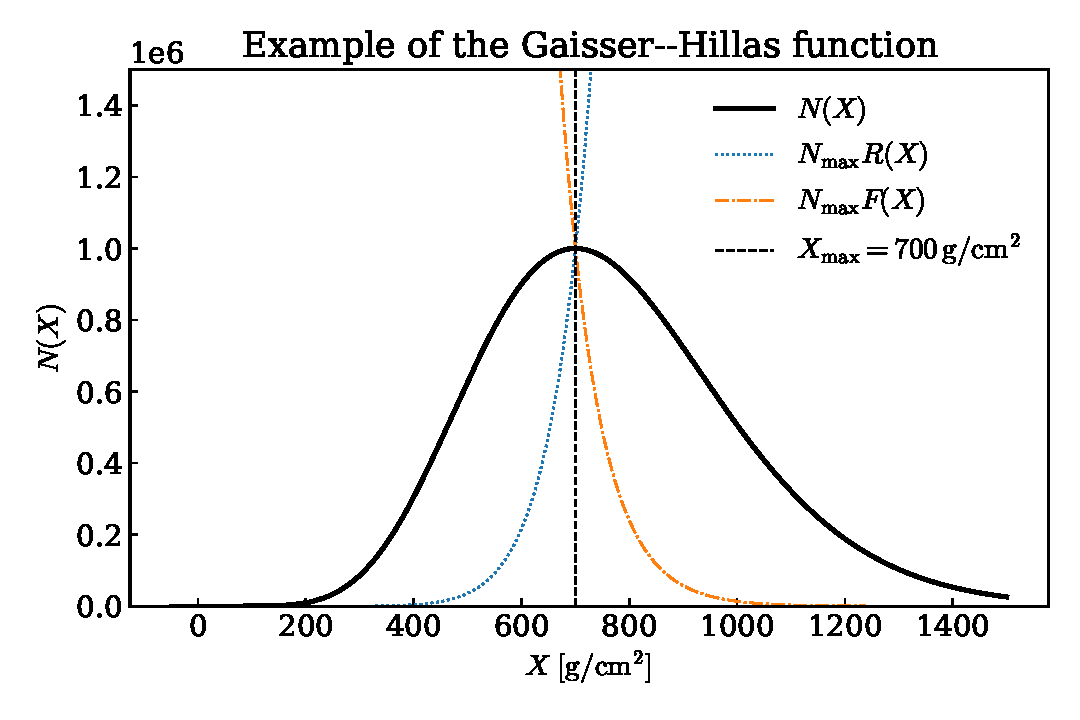
\includegraphics[width=0.75\hsize]{fig/gh.pdf}
    \caption{Gaisser--Hillas 関数の例。黒実線は \(N(X)\)、青点線は式~\eqref{eq:GH}のべき乗項 \(R(X)\) を \(N_{\max}\) 倍したもの、橙破線は指数関数項 \(F(X)\) を \(N_{\max}\) 倍したものを示す。\(N_{\max}=10^6\)、\(X_{\max}=700\ \mathrm{g\,cm^{-2}}\)、\(X_0^{\mathrm{GH}}=-50\ \mathrm{g\,cm^{-2}}\)、\(\Lambda=70\ \mathrm{g\,cm^{-2}}\) とした。}
    \label{fig:GH}
\end{figure}

\begin{description}
  \item[\(N_{\max}\)] プロファイルの最大値であり、全体の規格化を決める。
  \item[\(X_{\max}\)] プロファイルが最大となる大気深さを表す。
  \item[\(X_0^{\mathrm{GH}}\)] 立ち上がり側の有効な原点であり、必ずしも物理的な最初の相互作用点とは一致しない。
  \item[\(\Lambda\)] プロファイルの幅を決める形状パラメータであり、大きいほど分布は広くなる。
\end{description}

\subsubsection{極大構造と観測量}
式~\eqref{eq:GH}を \(X>X_0^{\mathrm{GH}}\) で対数微分すると、
\begin{equation}
  \frac{\mathrm d\ln N}{\mathrm dX}
  =\frac{X_{\max}-X}{\Lambda(X-X_0^{\mathrm{GH}})}
  \label{eq:dGH}
\end{equation}
となる。分母は正なので、\(X<X_{\max}\) で増加し、\(X>X_{\max}\) で減少する。\(X=X_{\max}\) を式~\eqref{eq:GH}へ代入すると \(N=N_{\max}\) となり、単峰の形状を確認できる。
この関数は縦方向プロファイルの形を表す経験式である。蛍光観測で再構成する量は粒子数そのものではなく大気へのエネルギー付与 \(\mathrm dE/\mathrm dX\) であり、そのプロファイルにも同じ関数形を用いる。

\subsection{大気蛍光とチェレンコフ光による縦方向発達の観測}\label{subsec:fluorescence}
空気シャワー中の荷電粒子は大気中の窒素分子を励起し、紫外域の蛍光を放出させる。
大気蛍光望遠鏡はこの光を追跡し、シャワー軸に沿った縦方向発達を再構成する~\cite{PDGCosmicRays,Stanev2004,TALEMassComposition2026}。
Fly's Eye は 1981 年に観測を開始し、大気蛍光法による宇宙線観測を初めて実用規模で実現した。この装置によって、UHECR のエネルギースペクトルと縦方向発達の測定が本格化した~\cite{BluemerEngelHorandel2009}。
その後、HiRes はステレオ観測と高分解能化を進め、Auger はハイブリッド観測によって大露出の地表アレイを蛍光観測で較正した~\cite{FlysEyeSpectrum1994,HiResGZK2008,AugerXmax2014}。
観測される蛍光光量は、粒子数 \(N(X)\) そのものではなく、その深さにおけるエネルギー付与 \(\mathrm{d}E/\mathrm{d}X\) と直接結び付いている。
縦方向プロファイルは GH 関数でよく記述できる。実際の解析では、同関数をプロファイルにフィットし、\(X_{\max}\) やシャワーサイズを表すパラメータを求める~\cite{GaisserHillas1977,PDGCosmicRays}。

空気シャワーは蛍光だけでなく、チェレンコフ光も放出する。
チェレンコフ光は、荷電粒子の速度が大気中における光の位相速度を超えたときに生じ、シャワー進行方向の近くに集中する。蛍光は、これとは異なり、ほぼ等方的に放出される。
縦方向発達の再構成では、蛍光、直接チェレンコフ光、大気中で散乱されたチェレンコフ光の寄与を光の伝搬とともに評価する。TALE では、チェレンコフ光を多く含む事象についても、その光量と角度依存を縦方向発達の情報として利用する~\cite{TALESpectrum2018,TALEMassComposition2026}。

この方法では、望遠鏡の視線方向と光の到来時刻からシャワー軸の位置と方向を決める。次に、大気中での吸収・散乱と各発光成分の寄与を含むモデルから、縦方向プロファイルを再構成する。蛍光収量は単位エネルギー付与あたりの蛍光光子数であり、発光量をエネルギー付与へ換算する基準となる。
再構成されたエネルギー付与プロファイルを大気深さにわたって積分すると、シャワーが大気中に失ったカロリメトリックエネルギーが得られる。
そこに大気へのエネルギー付与として回収されない不可視エネルギーの補正を加えることで、一次粒子エネルギーが推定される~\cite{PDGCosmicRays,Stanev2004,TALEMassComposition2026}。
不可視エネルギーにはニュートリノや地表へ到達する粒子が運ぶエネルギーが関係するが、ミューオンが大気中に付与したエネルギーまで不可視とするわけではない。
Tunka-133 の非結像型チェレンコフ観測では、地表の光密度と時間情報からエネルギーと発達を推定する。結像型の蛍光測定と同じ積分・較正手順ではなく、観測量と尺度の接続は表~\ref{tab:cosmic_ray_experiments}のように区別される~\cite{TunkaSpectrum2020}。
縦方向発達の記述では、簡略モデルと経験関数が異なる役割を担う。
Heitler モデルは、純粋な電磁シャワーに対して
\begin{equation}
  N_{\max}\propto E_0,
  \qquad
  X_{\max}\propto \ln E_0
\end{equation}
というスケーリングの物理的直観を与える~\cite{Heitler1944,PDGCosmicRays}。
Heitler--Matthews モデルは、これをハドロンシャワーへ拡張し、電子数、ミューオン数、質量組成への依存を半経験的に記述する~\cite{Matthews2005,Montanus2013}。
これらが物理的解釈を与える簡略モデルであるのに対し、Gaisser--Hillas 関数は観測された縦方向プロファイル全体を表す経験的なフィット関数である~\cite{GaisserHillas1977}。
\section{空気シャワーの横方向分布とシャワー前面}\label{sec:lateral_structure}
地上アレイでは、シャワー軸まわりの粒子分布と、粒子群の到来時刻から得られる時間構造を観測する。
前者を横方向分布として記述する。後者では、代表的な到来時刻から定める面をシャワー前面と呼び、その曲率と各位置での到来時刻分布の幅を区別する。

\subsection{横方向分布の定義と物理的起源}\label{subsec:lateral_definition}\label{subsec:why_lateral}
以下の軸対称な分布式では、シャワー軸に垂直な面での軸からの距離を \(r\) とし、面密度もこの面の単位面積あたりで定義する。鉛直シャワーでは地表面と一致するが、傾斜したシャワーでは投影と大気中の減衰を考慮して地表の観測量に対応づける必要がある。
このとき、半径 \(r\) における単位面積あたりの粒子密度を、一般に
\begin{equation}
  \rho(r)
\end{equation}
と書く。
ただし、実際には対象とする粒子種を明示し、電子成分を \(\rho_e(r)\)、ミューオン成分を \(\rho_\mu(r)\)、荷電粒子全体を \(\rho_{\mathrm{ch}}(r)\) のように書き分ける。

粒子の分布が軸対称であるなら、半径 \(r\) から \(r+\mathrm{d}r\) までの環状の領域に含まれる粒子数は
\begin{equation}
  \mathrm{d}N = 2\pi r\,\rho(r)\,\mathrm{d}r
\end{equation}
と表される。
後述する NKG 型関数と AGASA の経験式は、全粒子数そのものではなく、観測面での定義を対応づけた粒子密度分布 \(\rho(r)\) を記述する~\cite{KamataNishimura1958,Greisen1960,Yoshida1994}。

空気シャワーの横方向広がりを生む主因は、粒子種ごとに次のように整理できる。
\begin{itemize}
  \item 電磁成分では、低エネルギー電子・陽電子の多重クーロン散乱が横方向の広がりを強く支配する。
  \item 電子・光子は、制動放射や対生成を繰り返す過程そのものによっても角度広がりをもつ。
  \item ミューオンの広がりは、親パイオンや K 中間子が生成時にもつ横運動量、崩壊時の運動学、その後の散乱によって決まる。
\end{itemize}
電磁シャワーの横方向広がりは、主として低エネルギー電子のクーロン散乱で決まり、その代表尺度には Gert Moli\`ere に由来するモリエール半径が用いられる~\cite{PDGPassage,PDGCosmicRays}。
一方、ミューオン成分は生成時の横運動量を反映してより平坦な分布をもち、シャワー軸から遠い領域では電磁成分に対する割合が増す~\cite{Cazon2004}。
この違いは、後述するシャワー前面の構造にも影響する~\cite{Cazon2004}。

\subsection{モリエール半径}\label{subsec:moliere_radius}
モリエール半径は、電磁シャワーの横方向の代表スケールである。
電子・陽電子が散乱を繰り返す結果、電磁成分の大部分はこのスケールの内側に収まる~\cite{PDGPassage}。
モリエール半径を質量厚さで表した量を \(R_{\mathrm{M}}^{(X)}\) とすると、
\begin{equation}
  R_{\mathrm{M}}^{(X)} = X_0 \frac{E_s}{E^\mathrm{crit}}
\end{equation}
で与えられる。ここで \(E^\mathrm{crit}\) はその物質における電子の臨界エネルギーであり、\(E_s \simeq 21\ \mathrm{MeV}\) である~\cite{PDGPassage}。局所的な空気密度を \(\rho_{\mathrm{air}}\) とすると、幾何学的長さで表したモリエール半径は
\begin{equation}
  r_{\mathrm{M}}=\frac{R_{\mathrm{M}}^{(X)}}{\rho_{\mathrm{air}}}
\end{equation}
となる。一様な物質中の電磁シャワーでは平均的に、エネルギーの約 90\% が半径 \(r_{\mathrm{M}}\) の円柱内に、約 99\% が \(3.5r_{\mathrm{M}}\) の内側に含まれる~\cite{PDGPassage}。

第\ref{sec:longitudinal}節で述べたように、放射長 \(X_0\) は縦方向発達の代表尺度である。
これに対して、モリエール半径は横方向広がりの代表尺度であり、電磁成分の横方向分布を記述する際の自然なスケールを与える。
この対応のため、NKG 型の関数では \(r/r_{\mathrm{M}}\) のような無次元半径が基本変数として現れる~\cite{KamataNishimura1958,Greisen1960}。

モリエール半径を幾何学的長さ \(r_{\mathrm{M}}\) で表すと、その値は局所的な空気密度に依存する。
空気が薄いほど、同じ質量厚さに対応する幾何学的距離は大きくなるので、モリエール半径をメートルで表した値は高度とともに大きくなる。
PDG の乾燥空気（1 気圧）の表では、空気に対する質量厚さ表示のモリエール半径は \(R_{\mathrm{M}}^{(X)} \simeq 8.8\ \mathrm{g\,cm^{-2}}\) と与えられている~\cite{PDGAir}。
AGASA では、横方向分布式の半径スケールとして、Akeno 観測高度に対し「観測高度より 2 放射長上空」で定義されたモリエール単位 \(R_M\) を用い、その値を
\begin{equation}
  R_M = 91.6\ \mathrm{m}
\end{equation}
としている~\cite{Yoshida1994,Takeda2003}。
幾何学的長さで表したモリエール半径は、観測高度に依存する。

ただし、大気中では密度が高度とともに変わるため、局所密度から求めた半径一つでシャワー全体を厳密に表せるわけではない。モリエール半径は電磁成分の代表スケールとして用いる。
実際の空気シャワー全体の横方向分布には、ハドロン成分やミューオン成分が混ざり、さらに実験では検出器応答も重なる。
したがって、空気シャワー全体の横方向分布はモリエール半径だけでは決まらず、実験では検出器応答を含む経験的な分布関数が用いられる~\cite{Yoshida1994,Takeda2003}。

\subsection{電子成分の横方向分布と NKG 型の考え方}\label{subsec:nkg}
電磁成分の横方向分布を表す古典的な関数として、Jun Nishimura、Koichi Kamata、Kenneth Greisen に由来する Nishimura--Kamata--Greisen (NKG) 型の分布が広く用いられる~\cite{KamataNishimura1958,Greisen1960}。
代表的には、電子成分の面密度を
\begin{equation}
  \rho_e(r)
  =
  \frac{N_e}{r_{\mathrm{M}}^2}
  C(s)
  \left(\frac{r}{r_{\mathrm{M}}}\right)^{s-2}
  \left(1+\frac{r}{r_{\mathrm{M}}}\right)^{s-4.5}
  \label{eq:nkg}
\end{equation}
のように書く。
ここで \(N_e\) は観測深さにおける電子数、\(r_{\mathrm{M}}\) は横方向スケール、\(s\) はシャワー年齢である。規格化定数 \(C(s)\) は
\begin{equation}
  C(s)=\frac{\Gamma(4.5-s)}{2\pi\,\Gamma(s)\Gamma(4.5-2s)}
\end{equation}
であり、\(0<s<2.25\) の範囲では、式~\eqref{eq:nkg}を面積積分すると \(N_e\) が得られる。
この式から分かるように、NKG 型では
\begin{itemize}
  \item \(N_e\) が分布の規格化を決める。
  \item \(r_{\mathrm{M}}\) が横方向の広がりの尺度を決める。
  \item \(s\) が中心付近と外側の勾配を含む分布形状を決める。
\end{itemize}
NKG 型は、電磁成分の横方向分布を理解するための基準形である。AGASA では、同様に中心からの距離で粒子密度を表しつつ、地上アレイの測定に合わせた修正 Linsley 型の経験式を用いる。

\subsection{AGASA の横方向分布とエネルギー推定}\label{subsec:agasa_ldf}
広大な地上アレイは、シャワー軸から数百 \(\mathrm{m}\) ないし数 \(\mathrm{km}\) 離れた領域の粒子密度を測定する。
この距離範囲では、遠距離側の減衰と天頂角依存を取り入れた経験式が用いられる。
AGASA では、荷電粒子密度に対して John Linsley に由来する修正 Linsley 型の式
\begin{align}
  \rho_{\mathrm{ch}}(r,\theta)
  &=
  A
  \left(\frac{r}{R_M}\right)^{-\alpha}
  \left(1+\frac{r}{R_M}\right)^{-(\eta(\theta)-\alpha)}
  \left\{1+\left(\frac{r}{1000\,\mathrm{m}}\right)^2\right\}^{-\delta},
  \label{eq:agasa_ldf}
  \\
  \alpha &= 1.2,\qquad
  \delta = 0.6,\qquad
  R_M = 91.6\ \mathrm{m}, \nonumber\\
  \eta(\theta)
  &= (3.97\pm0.13) - (1.79\pm0.62)(\sec\theta-1) \nonumber
\end{align}
が用いられる~\cite{Teshima1986,Yoshida1994}。
ここで \(A\) は規格化を決めるフィットパラメータであり、一次粒子の質量数とは異なる。\(R_M\) は Akeno で定義されたモリエール単位である。これらの係数は AGASA の観測条件に基づく歴史的な具体例であり、TALE-SD の分布関数を規定する値ではない。

この式は、シャワー軸近傍から地上アレイが実際にサンプリングする遠距離側まで、荷電粒子密度を安定に記述する。
とくに
\begin{itemize}
  \item \(\left(r/R_M\right)^{-\alpha}\) が中心付近の勾配を与える。
  \item \(\left(1+r/R_M\right)^{-(\eta-\alpha)}\) が中間距離での落ち方を与える。
  \item \(\left\{1+(r/1000\,\mathrm{m})^2\right\}^{-\delta}\) が遠距離側の追加減衰を与える。
\end{itemize}
という分担になっている。

AGASA では、この分布をフィットして \(r=600\ \mathrm{m}\) における粒子密度 \(S(600)\) を求め、一次粒子エネルギーの推定に用いる~\cite{Takeda2003}。

電子成分はシャワー軸付近で卓越しやすいのに対し、ミューオン密度 \(\rho_\mu(r)\) はより平坦な横方向分布をもつ。荷電粒子密度 \(\rho_{\mathrm{ch}}(r)\) は電子・陽電子とミューオンを含み、シンチレータ信号 \(S(r)\) は、光子が検出器内で生成する荷電粒子や検出器応答の影響も受ける。
このため、理論的な電子密度 \(\rho_e(r)\) は、実験で扱う \(S(r)\) や \(\rho_{\mathrm{ch}}(r)\) と一般には一致しない。
地上アレイで用いられる横方向分布式は、純粋な電磁成分ではなく、検出器が実際に記録する信号の分布を表す~\cite{Teshima1986,Yoshida1994,Takeda2003,Cazon2004}。

\subsection{シャワー前面と到来方向再構成}\label{subsec:shower_front}
地上アレイでは、粒子密度に加えて到来時刻がシャワーの幾何を制約する。
シャワー前面は理想化すれば平面に近いが、実際には曲率と有限の時間幅をもつ。
AGASA 型の解析では、接平面の伝播時刻 \(T_f\) に対する平均遅れ \(T_d\) と、時間分布の幅 \(T_s\) を用いて前面構造を表す~\cite{LinsleyScarsi1962,Teshima1986,Takeda2003}。

粒子は同じ生成点から同じ経路を飛ぶわけではない。
生成高度の違い、散乱、横方向運動量、速度の違いによって、軸から遠い粒子ほど平均的に長い経路を通り、遅れて地上へ到来しやすい。
その結果、シャワー軸付近では粒子が先に到来し、軸から遠いほど遅れる。地上で観測されるシャワー前面は、平面から遅れ側へ湾曲する~\cite{LinsleyScarsi1962,Cazon2004}。

この遅れは経験式で表され、到来方向やコア位置の再構成に利用される。
広い地上アレイでは、まず平面近似から方向の初期値を求める。その後、曲率と時間幅を取り入れて再構成を改善する手順がよく用いられる~\cite{LinsleyScarsi1962,Teshima1986,Takeda2003}。

ミューオンは比較的高エネルギーで直進性が高く、生成後の散乱も小さいため、シャワー前面の早い部分を形成しやすい。
これに対して、電子・光子成分は散乱と電磁カスケードの影響を強く受け、時間幅が大きくなりやすい。
そのため、遠距離や大天頂角ではミューオン優勢となり、シャワー前面の見え方も変化する~\cite{Cazon2004}。

地上アレイ解析では、横方向分布を主としてコア位置とシャワーサイズの推定に、シャワー前面の時間構造を主として到来方向の再構成に用いる。
実際の再構成では、この 2 つを同時に用いて、イベントの幾何とエネルギーを決める~\cite{Takeda2003}。

\section{一次エネルギーの推定と較正方法}\label{sec:energy_calibration}
\subsection{観測量とエネルギーへの換算}
地表検出器が測る信号 \(S(r)\)、地表でのチェレンコフ光密度、光学観測で再構成する縦方向発達は、いずれも一次エネルギーそのものではない。エネルギーの推定には、観測量からエネルギーへの写像と、その尺度を定める較正が必要となる。写像の形を実測から求める方法と、モンテカルロシミュレーション（MC）から与える方法では、観測データによって制約する部分が異なる。
地表信号の大きさは、同じエネルギーでも天頂角と発達段階によって変化する。まずこの依存性を扱い、その後に信号と一次エネルギーを対応づける、という二つの操作を区別する。

\subsection{CIC による天頂角補正と実測による較正}
Constant intensity cut（CIC）法は、到来強度がほぼ等方的であると仮定し、同じ積分強度に対応する信号を天頂角ごとに比較して減衰曲線を求める方法である。これにより地表信号を基準角に換算するが、CIC だけで絶対エネルギースケールを定めるわけではない。
Auger SD433 では、軸から \(300\ \mathrm m\) の信号 \(S(300)\) を天頂角 \(30^\circ\) へ補正した \(S_{30}\) を用いる。その後、SD750 と同時に観測した事象を用いて
\begin{equation}
  E=A_{\mathrm{cal}}\left(\frac{S_{30}}{S_0}\right)^{B_{\mathrm{cal}}}
  \label{eq:measured_energy_calibration}
\end{equation}
という関係を適合する。\(S_0\) は基準信号、\(A_{\mathrm{cal}}\) はエネルギーの次元をもつ規格化、\(B_{\mathrm{cal}}\) は無次元の指数である。SD750 のエネルギーは蛍光検出器（FD）に較正されているため、SD433 の尺度も SD750 を介して FD へ接続される~\cite{AugerSD4332023}。
この解析では \(S_0=30\ \mathrm{VEM}\) に対して、\(A_{\mathrm{cal}}=(117.0\pm0.4)\ \mathrm{PeV}\)、\(B_{\mathrm{cal}}=0.963\pm0.003\) が得られている。VEM は鉛直に通過するミューオンに対応する信号の単位である。適合には両アレイの分解能、スペクトル形状、\(E_{750}>100\ \mathrm{PeV}\) の選択条件と信号間の相関が含まれる~\cite{AugerSD4332023}。規格化に加えて傾きもデータから求める点が、次に述べる定数係数のみの較正とは異なる。
FD に接続した尺度にも、蛍光収量、大気透過、検出器の光学較正、不可視エネルギー補正などの不確かさが残る~\cite{AugerSecondKnee2021}。CIC と実測の較正を行ったことだけから、ハドロン相互作用モデルに対する依存がすべて消えるとはいえない。

図~\ref{fig:auger433_calibration}は、この実測による較正を示す。指数 \(B_{\mathrm{cal}}\neq1\) は信号とエネルギーという異なる量の関係を表し、それだけで再構成エネルギーの非線形な偏りを意味するわけではない。
\begin{figure}[htb]
  \centering
  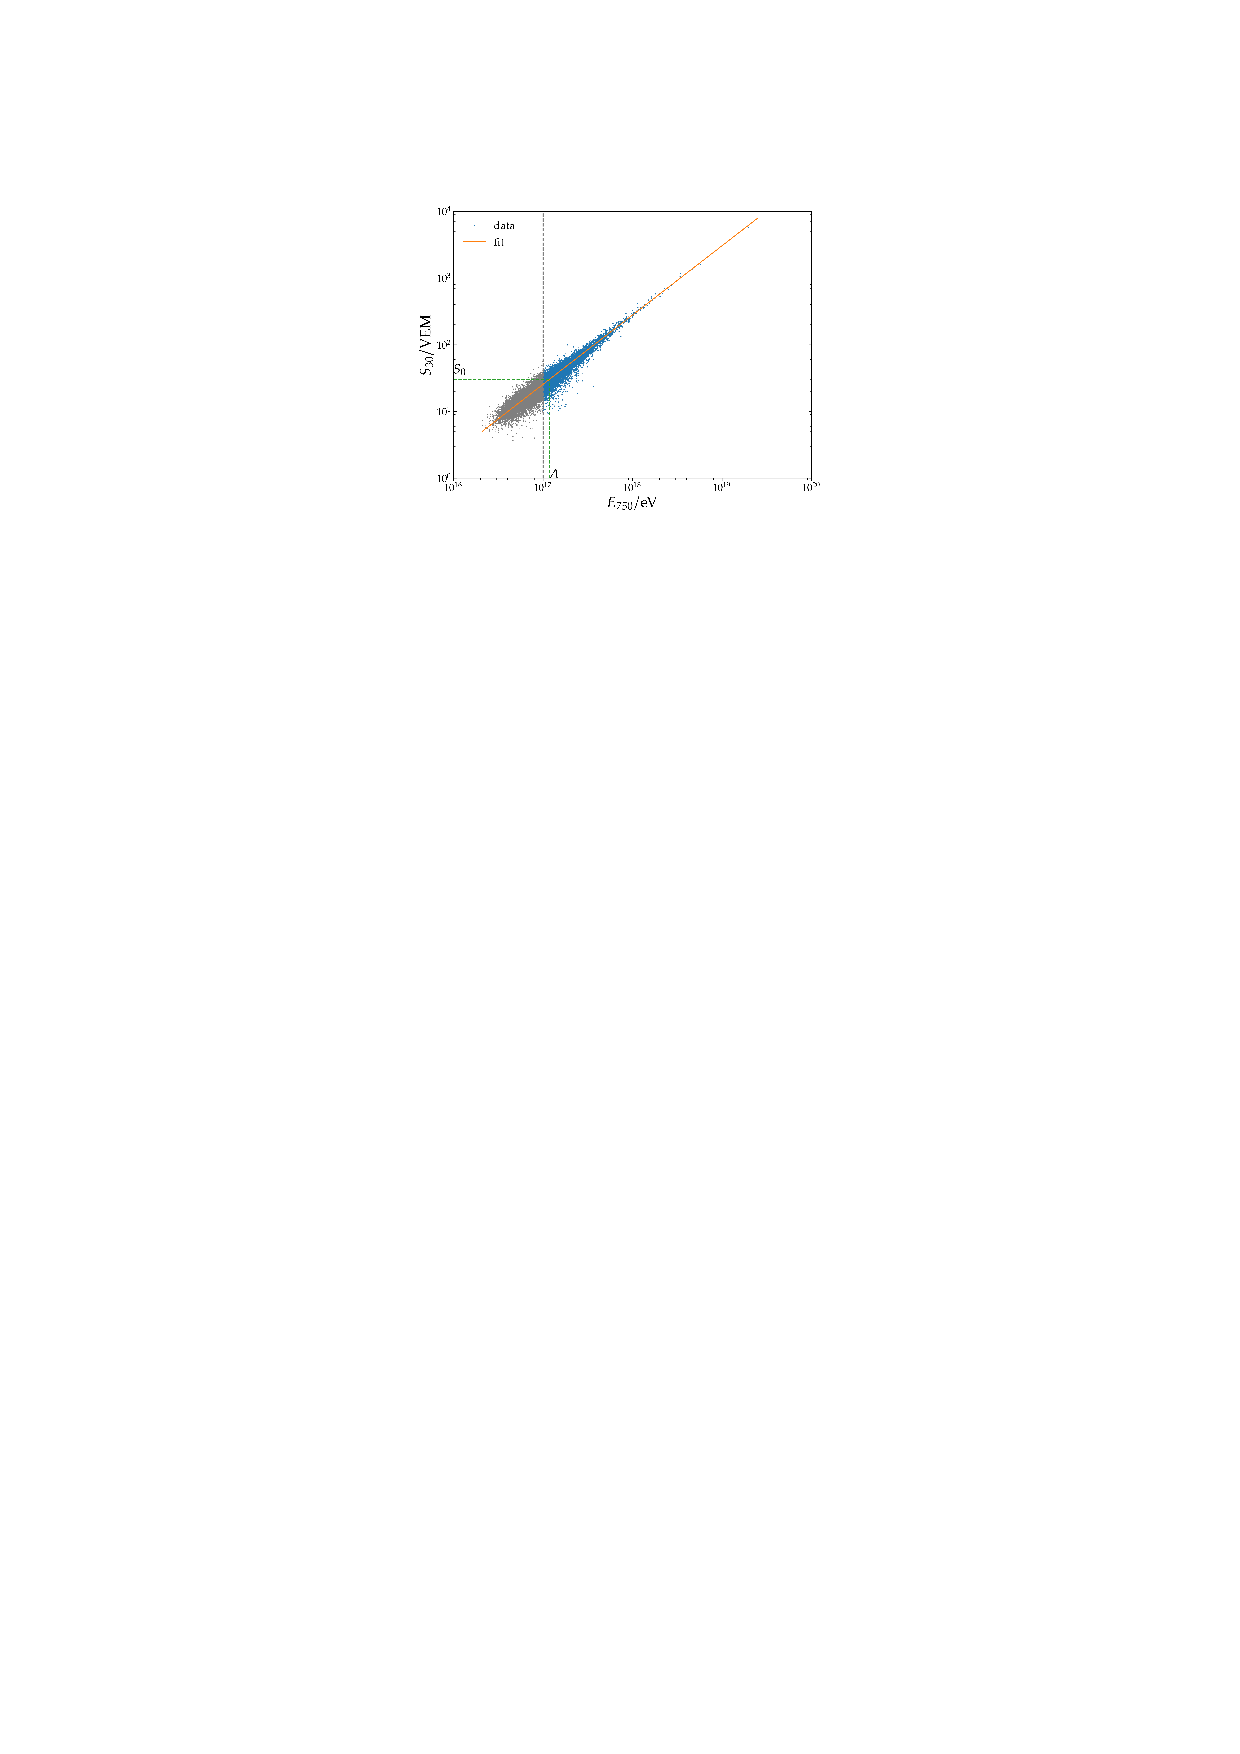
\includegraphics[width=0.62\hsize]{fig/auger-sd433-2023-fig4.pdf}
  \caption{Auger SD433 と SD750 の同時観測による \(S_{30}\) とエネルギーの較正。青点は \(E_{750}>100\ \mathrm{PeV}\) の較正事象、灰色点はその閾値より下の事象、橙線は規格化と指数を求めた適合を示す。緑線は基準信号とそれに対応するエネルギーを表す。これは CIC 曲線ではなく、その補正後の信号をエネルギーへ換算する関係である。G. Brichetto Orquera for the Pierre Auger Collaboration, PoS(ICRC2023)398, Fig.~4 より転載~\cite{AugerSD4332023}。\href{https://creativecommons.org/licenses/by-nc-nd/4.0/}{CC BY-NC-ND 4.0}。図の内容は変更していない。}
  \label{fig:auger433_calibration}
\end{figure}

\subsection{MC による換算関係と定数係数の較正}
MC で作成した対応表や関数からエネルギーを求め、その全体に定数を掛ける方法は、例えば
\begin{equation}
  E_{\mathrm{rec}}=C\,F_{\mathrm{MC}}(S_{600},\theta)
  \label{eq:mc_lookup_calibration}
\end{equation}
と書ける。ここで \(S_{600}\) は軸から \(600\ \mathrm m\) の信号、\(\theta\) は天頂角、\(F_{\mathrm{MC}}\) はエネルギーの次元をもつ MC の換算関係、\(C\) は無次元の定数である。この式は方法を比較するための一般形である。
同時観測などから \(C\) を決めると、比較範囲における平均的な尺度の差を補正できる。しかし、信号に対する傾きや曲率は \(F_{\mathrm{MC}}\) に由来するため、較正範囲内でもエネルギーに依存する残差があり得る。平均エネルギー差が小さいことと、スペクトル形状が正しく再構成されることは、異なる検証を要する。
陽子と鉄を仮定した推定結果の比較は、その二つの組成仮定に対する感度を調べるものである。両者が近いだけでは、両仮定に共通するハドロン相互作用や検出器応答の誤差まで小さいとは結論できない。

\subsection{ミューオン信号の差が残すエネルギー依存}
地表の全信号を電磁成分とミューオン成分の和として考える。固定した幾何条件と組成について、電磁信号は MC が正しく記述し、ミューオン信号だけが異なると仮定すると、
\begin{equation}
  h(E)\equiv\frac{S_{\mathrm{data}}(E)}{S_{\mathrm{MC}}(E)}
  =1+f_\mu(E)\{r_\mu(E)-1\}
  \label{eq:muon_signal_ratio}
\end{equation}
となる。ここで \(f_\mu=S_{\mu,\mathrm{MC}}/S_{\mathrm{MC}}\) は MC の全信号に占めるミューオン信号の割合、\(r_\mu=S_{\mu,\mathrm{data}}/S_{\mu,\mathrm{MC}}\) はその実測と MC の比である。これらは粒子数やミューオン密度の比とは一般に異なる。
対象範囲で \(S_{\mathrm{MC}}\propto E^\alpha\)（\(\alpha>0\)）とし、基準エネルギー \(E_*\) で定数較正を行うと、逆関数による換算から
\begin{equation}
  \frac{E_{\mathrm{rec}}}{E}
  \simeq\left[\frac{h(E)}{h(E_*)}\right]^{1/\alpha}
  \label{eq:residual_energy_bias}
\end{equation}
を得る。\(f_\mu\) または \(r_\mu\) がエネルギーによって変われば、定数較正後にも差が残る。この式は仮定を限定した説明用の近似であり、特定の検出器で測定した信号割合を与えるものではない。実際の応答には、組成、天頂角、軸からの距離、電磁成分の模型差も関係する。

\subsection{エネルギーの換算とスペクトル形状}
分解能を省き、エネルギー間の写像 \(E_{\mathrm{rec}}=g(E)\) が単調増加であるとする。同じ露出で事象数を保存すると、微分強度は
\begin{equation}
  J_{\mathrm{rec}}(E_{\mathrm{rec}})
  =J(E)\frac{\mathrm dE}{\mathrm dE_{\mathrm{rec}}}
  \label{eq:spectrum_energy_mapping}
\end{equation}
と変換される。定数倍率 \(E_{\mathrm{rec}}=kE\) の場合にも、\(J_{\mathrm{rec}}(E_{\mathrm{rec}})=J(E_{\mathrm{rec}}/k)/k\) である。純粋なべき乗則なら同じ表示エネルギーでの強度比は一定になるが、折れ曲がりを含むスペクトルでは一般に一定にならない。したがって、実験間の強度比がエネルギーによって変化することだけでは、エネルギー換算の非線形性は証明できない。一方、定数係数を較正したことだけから非線形な差を除外することもできない。
実測では、検出効率とエネルギー分解能を含めて期待事象数を評価する。方向と時間を積分した有効露出を \(\mathcal E(E)\)、選択された事象の条件付き応答を \(P(E_{\mathrm{rec}}\mid E)\) とすると、
\begin{equation}
  \frac{\mathrm dN}{\mathrm dE_{\mathrm{rec}}}
  =\int J(E)\,\mathcal E(E)\,P(E_{\mathrm{rec}}\mid E)\,\mathrm dE
  \label{eq:spectrum_response}
\end{equation}
と書ける。\(\mathcal E\) は検出・選択効率を含み、単位は \(\mathrm{m^2\,sr\,s}\) である。\(P\) は \(E_{\mathrm{rec}}\) について規格化した確率密度で、エネルギーの逆数の単位をもつ。\(J\) を \(\mathrm{eV^{-1}\,m^{-2}\,s^{-1}\,sr^{-1}}\) で表せば、両辺は \(\mathrm{eV^{-1}}\) となる。これらの量は必要に応じて核種ごとに評価し、強度を重みとして合計する。
検出閾値付近の効率変化とエネルギー区間間の事象移動は、折れ曲がりの位置と鋭さの推定に影響する。Auger SD433 では応答を通したスペクトルの予測をデータへ適合しており~\cite{AugerSD4332023}、TALE-SD と光学測定の比較でも、尺度と形状の双方について応答を考慮することが重要となる。

\backmatter
\cleardoublepage
\phantomsection
\addcontentsline{toc}{chapter}{参考文献}
\renewcommand{\refname}{参考文献}
\bibliographystyle{jhep}
\bibliography{main}

\end{document}
